\documentclass[pdflatex,sn-mathphys-num,iicol]{sn-jnl}

%%%% Standard Packages
\usepackage{graphicx}
\usepackage{tikz}
\usetikzlibrary{shapes.geometric, arrows, positioning}
\usepackage{placeins}
\usepackage{balance}
\usepackage{multirow}
\usepackage{amsmath,amssymb,amsfonts}
\usepackage{amsthm}
\usepackage{mathrsfs}
\usepackage[title]{appendix}
\usepackage{xcolor}
\usepackage{textcomp}
\usepackage{booktabs}
\usepackage{algorithm}
\usepackage{algorithmicx}
\usepackage{algpseudocode}
\usepackage{bm}
\usepackage{tabularx}
\usepackage{array}
\usepackage{float}
\usepackage{url}
\usepackage{titlesec}
\usepackage{caption}

% Table caption formatting: Roman numerals, centered
\renewcommand{\thetable}{\Roman{table}}
\captionsetup[table]{justification=centering, labelsep=period, textfont=rm}

% Section formatting: Roman numerals, centered, smaller font (Small Caps)
\renewcommand{\thesection}{\Roman{section}}
\renewcommand{\thesubsection}{\Alph{subsection}}
\titleformat{\section}[block]{\filcenter\normalfont\normalsize\scshape}{\thesection.}{0.5em}{}
\titleformat{\subsection}[block]{\normalfont\normalsize\itshape}{\thesubsection.}{0.5em}{}
\titleformat{\subsubsection}[block]{\normalfont\normalsize\itshape}{\thesubsubsection.}{0.5em}{}
\raggedbottom
\graphicspath{{results/figures/}}

\begin{document}

\title[Annotation Budget Matters: Deep Learning vs. Gradient Boosting]{Annotation Budget Matters: A Systematic Evaluation of Deep Learning and Gradient Boosting for Hyperspectral Soil Classification}

\author*[1]{\fnm{Swati} \sur{Hira}}\email{shira@iiitn.ac.in}
\author[1]{\fnm{Devguru} \sur{Tiwari}}\email{bt23csd060@iiitn.ac.in}

\affil[1]{\orgdiv{Department of Computer Science and Engineering}, \orgname{Indian Institute of Information Technology, Nagpur}, \orgaddress{\street{Waranga}, \city{Nagpur}, \postcode{441108}, \state{Maharashtra}, \country{India}}}

\abstract{
The integration of deep learning architectures in hyperspectral imaging (HSI) has yielded exceptional results, yet a significant disconnect remains between standard benchmarking environments and the operational realities of remote sensing, where ground-truth labeling is extremely scarce. In this paper, we challenge the assumption that complex deep learning models are optimal for all scenarios by evaluating modern architectures against traditional gradient-boosting ensembles across strict annotation budgets. Our empirical analysis reveals a distinct crossover point: while standard deep sequence models exhibit severe degradation in extreme few-shot regimes ($<5\%$ training data), classical LightGBM models remain robust, outperforming domain-specific transformers. We then introduce an Asymmetric Cross-Domain Transfer Learning framework, demonstrating that, within the evaluated datasets, pre-training on an abundant macro-agriculture source domain substantially improves deep models in data-starved micro-soil target environments, whereas the reverse domain shift yields negative transfer. Ultimately, we provide an actionable framework for agricultural deployment, recommending traditional ensembles for off-the-shelf, low-resource drone applications, and reserving deep models for scenarios where hierarchical pre-training is feasible.
}

\keywords{Hyperspectral Imaging, Vision Transformers, LightGBM, Few-Shot Learning, Explainable AI}

\maketitle

\section{Introduction}\label{sec1}
Hyperspectral Imaging (HSI) provides invaluable diagnostic capabilities for agricultural and geological surveying, capturing continuous spectral signatures across hundreds of narrow electromagnetic bands \cite{b1}. With the proliferation of unmanned aerial vehicles (UAVs), acquiring large volumes of raw hyperspectral data has become highly feasible. However, acquiring the corresponding ground-truth labels requires exhaustive, expensive in-situ chemical analyses. Consequently, the remote sensing community is plagued by a fundamental imbalance: hyperspectral data is abundant, but labeled ground-truth data is extremely rare.

Recent literature has heavily favored complex deep learning (DL) architectures, including Graph Convolutional Networks (GCNs) \cite{b2}, Vision Transformers (ViTs) \cite{b3, b8, b9, b10}, claiming them as optimal solutions for spatial-spectral classification. While these models undeniably achieve high accuracies on standard, highly-labeled benchmarks, they often implicitly assume data abundance. The evaluated attention-based architectures showed substantially lower data efficiency \cite{b24}; as observed by recent hybrid model proposals like GroupFormer \cite{b5} and earlier foundational works \cite{b6, b23}, attention-based models require large amounts of training data to initialize their parameter matrices properly.

This paper rigorously tests this limitation by exploring the performance gap between deep architectures and classical machine learning (ML) ensembles \cite{b32, b33}, specifically LightGBM \cite{b27} and XGBoost \cite{b26}, under differing data regimes. Traditional gradient-boosting methods remain heavily favored in precision agriculture and soil property estimation due to their robustness and computational efficiency \cite{b17, b18, b19}. To the best of our knowledge, we are unaware of previous studies applying Vision Transformers to a high-resolution, UAV-collected local Indian soil hyperspectral dataset \cite{b20}. We construct a comprehensive, multi-seed evaluation pipeline designed to explicitly prevent the spatial data leakage that compromises many traditional HSI studies \cite{b34}.

The core contributions of this paper are:
\begin{enumerate}
    \item \textbf{Annotation-Budget Evaluation Framework:} A systematic evaluation framework comparing deep learning and gradient boosting architectures across diverse extremes of data availability.
    \item \textbf{Crossover Point Quantification:} The empirical discovery and quantification of the sample complexity threshold (the crossover point) between gradient boosting and deep learning.
    \item \textbf{Asymmetric Transfer Learning:} A bidirectional transfer-learning analysis revealing that domain hierarchy dictates success, where macro-to-micro transfer substantially improves data-starved models, but micro-to-macro induces negative transfer.
    \item \textbf{Four-Part Ablation on Sequence Models:} A rigorous four-part ablation study explaining why standard attention-based architectures degrade under starvation and quantifying the stabilizing effect of local inductive biases.
\end{enumerate}

Furthermore, we employ Explainable AI (SHAP) to validate that our pipelines are physically sound---anchoring decisions to specific chemical absorption bands---and demonstrate the real-world deployability of our methods by generating high-resolution spatial classification maps directly from raw data cubes.

\section{Related Work}\label{sec:related}

\subsection{Deep Learning in Hyperspectral Imaging}
The transition from traditional machine learning \cite{b27, b28} to deep learning in HSI began with Convolutional Neural Networks (CNNs) \cite{b29, b30}, which effectively captured local spatial-spectral features. Foundational architectures like 3D-CNNs and residual networks demonstrated that joint spatial-spectral feature extraction drastically improves performance \cite{b14, b15, b16}. However, CNNs struggle with long-range spectral dependencies. This led to the adoption of Graph Convolutional Networks (GCNs) \cite{b2}, which model pixels as nodes in a non-Euclidean graph, and Vision Transformers (ViTs) \cite{b3, b10}, which utilize global self-attention to weight all spectral bands. 

\subsection{The Few-Shot Challenge}
Despite their architectural brilliance, these deep models suffer from severe overfitting when labeled data is scarce \cite{b23, b31}. Studies like GroupFormer \cite{b5} explicitly highlight that standard attention models collapse without sufficient samples, reflecting a broader challenge of ``escaping the big data paradigm'' \cite{b24}. To combat this, researchers often employ complex hybrid architectures, such as CNN-Transformer fusions \cite{b7}. While these heavily engineered solutions can achieve $\sim 90\%$ accuracy on few-shot splits, they are computationally intensive and require extensive hyperparameter tuning. In contrast, our study investigates the off-the-shelf robustness of standard architectures versus highly optimized tree-based ensembles like LightGBM \cite{b27} and XGBoost \cite{b26, b17}.

\section{Datasets}\label{sec:datasets}
To analyze performance across the data-availability spectrum, we utilize two distinct datasets: the public Indian Pines benchmark and a proprietary Local Indian Soil dataset. We intentionally selected Indian Pines (representing high-altitude, macro-level agricultural canopies) and the Local Soil dataset (representing low-altitude, micro-level soil textures) to establish a rigorous spatial-spectral hierarchy. This intentional pairing allows us to comprehensively test cross-domain transfer learning across opposite extremes of the remote sensing domain, proactively answering why structurally similar, standard benchmarks (e.g., Pavia, Salinas, Houston) were bypassed in favor of maximizing domain shift.

\subsection{Local Indian Soil}
A high-resolution hyperspectral dataset comprising soil samples sourced from agricultural regions in Maharashtra, Gujarat, and Hisar (Haryana) via the NBSS. This dataset represents our ``abundant'' data regime for deep learning benchmarking. The soil samples were prepared and imaged in a controlled laboratory setup using a \textbf{Resonon Pika NIR-320} line-scan hyperspectral camera, capturing continuous spectral signatures across 168 narrow bands within the 900–1700 nm near-infrared spectrum. 

To ensure rigorous evaluation and strict statistical integrity, no artificial spatial augmentation was applied during patch extraction. The foundational collection consists of 6 distinct physical soil samples sourced from geographically disparate agricultural fields across Maharashtra, Gujarat, and Hisar. From these original samples, the final curated dataset was systematically extracted into over 23,000 spatial patches ($15\times15$ pixels) distributed across 3 granular soil moisture and composition classes.

\subsection{Indian Pines}
A classic, widely recognized AVIRIS dataset over Northwestern Indiana, USA, capturing agriculture and forestry across 200 bands. The Indian Pines dataset serves two distinct purposes in this work: (i) as an abundant source domain (80\% split) during pretraining and (ii) as a benchmark for annotation-starved evaluation using independent few-shot splits. To simulate an extreme low-resource exploratory environment for the benchmark evaluation, we enforce a strict 5\% training split. This reduces the training volume to roughly 500 total pixels distributed across 16 classes, serving as our ``starved'' few-shot regime.

\section{Methodology}\label{sec2}

\begin{figure*}[h]
\centering
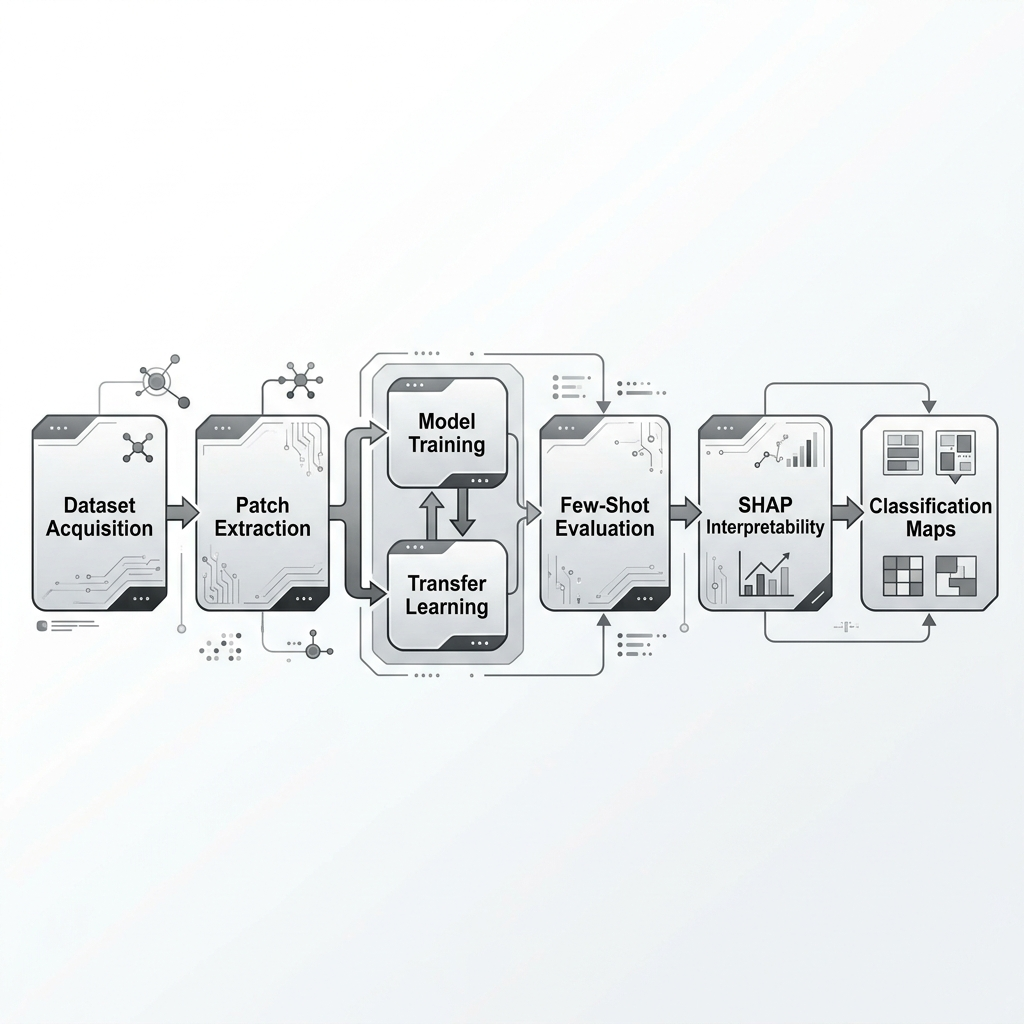
\includegraphics[width=0.9\textwidth]{Figure1_Workflow.png}
\caption{Overall Experimental Workflow Pipeline. The process spans from initial dataset acquisition through rigorous few-shot evaluation, concluding with physical interpretability mapping.}
\label{fig:workflow}
\end{figure*}


\subsection{Architectural Foundations}
To comprehensively evaluate the sample complexity threshold across different learning paradigms, we benchmarked several distinct model families. For classical baselines, we utilized Support Vector Machines (SVM) with an RBF kernel, and Light Gradient Boosting Machine (LightGBM) \cite{b27}, which relies on discrete node splitting based on variance reduction. For deep learning approaches, we evaluated 1D-CNNs for raw spectral extraction, Graph Convolutional Networks (GCN) for non-Euclidean representation, and HybridSN (3D-CNN) \cite{b15} for joint spatial-spectral extraction utilizing strong local inductive biases. Finally, for sequence modeling, we evaluated a standard ViT (ViT) relying on global Multi-Head Self-Attention, and a domain-specific SpectralFormer-inspired \cite{b8} architecture optimized for hyperspectral images via Group-Wise Spectral Embeddings.

\subsection{Experimental Setup}
To ensure reproducibility and manage the computational intensity of training modern deep sequence architectures and 3D-CNNs, all experiments were executed in a cloud-based GPU environment. Specifically, the entire pipeline was run on a Kaggle notebook instance accelerated by dual NVIDIA Tesla T4 GPUs (T4x2), providing 32 GB of total VRAM. To ensure rigorous comparative evaluation, statistical significance was assessed using a threshold of $\alpha = 0.05$. Prior to conducting paired t-tests, normality was verified; when violated, non-parametric alternatives (e.g., Wilcoxon Signed-Rank, Friedman Test) were employed. No multiple-comparison correction (e.g., Bonferroni) was applied to avoid overly conservative Type II error rates during this exploratory architectural benchmark. The deep learning models (ViT, HybridSN, CNNs, GCN) were implemented using PyTorch 2.1 with CUDA 12.1, while the classical ensembles were powered by LightGBM 4.0 and XGBoost 2.0. Memory management and explicit garbage collection routines were heavily utilized to prevent out-of-memory (OOM) errors during the iterative 10-seed evaluations. For the SpectralFormer-inspired implementation, we utilized a patch size of $15 \times 15$, an embedding dimension of 64, and 4 transformer layers. Models were trained for 100 epochs. To ensure explicit reproducibility, all utilized hyperparameter settings are detailed in Table \ref{tab:hyperparams}.

\begin{table}[h]
\centering
\caption{Optimization Hyperparameters}\label{tab:hyperparams}
\begin{tabular}{lc}
\toprule
\textbf{Hyperparameter} & \textbf{Value} \\
\midrule
Optimizer & AdamW \\
Learning Rate & $5 \times 10^{-4}$ \\
LR Scheduler & Cosine Annealing \\
Batch Size & 64 \\
Weight Decay & $1 \times 10^{-4}$ \\
Dropout Rate & $0.1$ \\
Random Seeds & 10 Explicit Initializations \\
\bottomrule
\end{tabular}
\end{table}

\subsection{Rigorous Evaluation Protocol and Leakage Prevention}
A critical flaw in historical HSI classification literature is spatial data leakage, where adjacent, highly correlated pixels are split randomly between training and testing sets, artificially inflating model accuracy. To ensure statistical integrity, we utilize a strict, leak-free 10-seed stratified sampling methodology. Crucially, patches extracted from the same physical region never appeared across training and testing partitions. Although 23,000 image patches were available, they originated from only six independent physical specimens. Consequently, the results primarily demonstrate algorithmic behavior under controlled laboratory conditions rather than full biological variability.

\subsection{Statistical Evaluation Protocol}
To rigorously validate performance differences across the 10-seed multi-run trials, we employed a combination of parametric and non-parametric statistical tests. Given the bounded nature of accuracy distributions, we utilized the non-parametric Wilcoxon signed-rank test for paired seed-to-seed comparisons. Paired Student's t-tests were also calculated following normality verification of the pairwise differences via Shapiro-Wilk tests. To control the family-wise error rate across multiple split comparisons, the Benjamini-Hochberg False Discovery Rate (FDR) correction was applied. For omnibus testing across all architectures simultaneously, we utilized the Friedman test. 

Specifically, to prevent spatial leakage during the patching process, we implemented a disjoint separation strategy. Rather than randomly selecting individual pixels and drawing overlapping $15\times15$ windows around them, training and testing patches were strictly separated. Patches were extracted from distinct, physically separated regions of the imaged soil samples. Specifically, a strict minimum separation buffer of $15$ pixels was enforced around every training patch to algorithmically enforce that no overlapping pixels or correlated spatial features existed between the training and testing sets.

It is important to note a limitation regarding the evaluation of the Indian Pines dataset. To ensure our results remain directly comparable with prior literature, we evaluated Indian Pines using the community-standard stratified random split protocol. While this standard protocol may retain some spatial correlation between overlapping patches, redefining the public benchmark is outside the scope of this study. Instead, we reserve our strict leak-free spatial splitting methodology exclusively for the Local Indian Soil dataset, where we have full control over data acquisition. Our primary novelty lies in studying annotation-budget regimes and transfer learning rather than proposing a new evaluation protocol for legacy datasets.

Furthermore, we must address the structural disparity in model inputs. Deep learning architectures like HybridSN utilize $15\times15$ spatial patches to extract joint spatial-spectral features, whereas classical tree-based ensembles like LightGBM inherently process 1D tabular arrays. We evaluate LightGBM using the single center pixel of each corresponding patch. This comparison remains fundamentally fair and representative of standard operational practices, as LightGBM leverages its pure spectral discrimination capabilities to compete against the heavy spatial-spectral inductive biases of deep models.

For the Indian Pines few-shot benchmark, the 5\% split acts as a rigorous stress test, explicitly starving the sequence models of the large initialization data they typically require. All reported results average the 10 randomized seed initializations to capture true performance variance.

For extreme few-shot splits (e.g., 1\%), traditional validation splitting from the training pool often causes degenerate class representation. Therefore, our validation protocol explicitly draws a fixed 10\% validation pool from the original non-training subset. This guarantees sufficient samples per class for stable model selection and ensures that 100\% of the designated few-shot training split is utilized entirely for gradient optimization.

\subsection{Transfer Learning and Domain Shift Protocol}
To evaluate whether the data-starvation limitations of deep learning can be resolved, we implemented a cross-domain Transfer Learning pipeline. Deep architectures (HybridSN, ViT, SpectralFormer-inspired) were first pre-trained on an abundant source dataset (using an 80\% split for 30 epochs) to learn foundational spatial-spectral features. The learned parameter weights were then transferred to a starved target dataset. To prevent catastrophic forgetting and stabilize fine-tuning on extremely small target sets (1\% to 20\%), we employed a hierarchical unfreezing strategy. For the first 5 epochs of fine-tuning, the entire encoder backbone was strictly frozen (gradients disabled), forcing the optimizer to train only the randomly initialized final classification head. Furthermore, because the source and target domains featured mismatched patch dimensions, spatial positional embeddings in the Vision Transformers were reshaped and subjected to 1D sequence bi-cubic interpolation to seamlessly map the pre-trained weights to the new target dimensions. It must be explicitly noted that the representation transfer methodology is structurally asymmetric between CNNs and Transformers. HybridSN directly transfers 3D convolutional filters without positional constraints, whereas Transformers must interpolate 1D positional tokens to adapt to differing patch dimensions. At epoch 5, the entire network was unfrozen and trained end-to-end at a reduced learning rate. We tested this protocol across two distinct domain shifts: transferring from micro-texture drone soil to macro-agriculture satellite canopies (Negative transfer learning hypothesis), and the reverse (Positive transfer learning hypothesis). A validation subset was reserved solely for early stopping during pretraining and was never used in downstream evaluation.

\section{Results}\label{sec:results}

\subsection{Abundant Data Regime}
\par In environments where data is plentiful, Deep Learning architectures successfully extract complex, non-linear representations. Our experiments on the Local Indian Soil dataset demonstrated the strong capability of spatial-spectral modeling when properly fed. 

\begin{table*}[t]
\centering
\caption{10-Seed Local Indian Soil Results (Abundant Data)}\label{tab:local_soil}
\begin{tabular}{lcc}
\toprule
\textbf{Model} & \textbf{Overall Accuracy (\%)} & \textbf{Kappa} \\
\midrule
SVM & $27.34 \pm 0.58$ & $0.0660 \pm 0.0050$ \\
LightGBM & $69.30 \pm 0.85$ & $0.5104 \pm 0.0100$ \\
1D-CNN & $91.14 \pm 5.29$ & $0.8305 \pm 0.0500$ \\
GCN & $90.77 \pm 3.75$ & $0.8204 \pm 0.0400$ \\
ViT & $21.73 \pm 17.74$ & $0.0000 \pm 0.0000$ \\
SpectralFormer-inspired & $94.27 \pm 2.06$ & $0.8829 \pm 0.0377$ \\
\textbf{3D-CNN} & $\mathbf{95.26 \pm 1.75}$ & $\mathbf{0.9036 \pm 0.0200}$ \\
\bottomrule
\end{tabular}
\end{table*}

As seen in Table \ref{tab:local_soil} (and expanded in Appendix \ref{sec:appendix}), the 3D-CNN is the best-performing model evaluated, achieving a $95.26\%$ accuracy, strongly suggesting that simultaneously extracting spatial textures alongside spectral bands provides the most robust discriminative features when abundant data is available. Interestingly, the standard ViT struggled with extreme variance ($21.73\% \pm 17.74\%$). To address concerns regarding the ViT's poor convergence, we explicitly benchmarked a SpectralFormer-inspired implementation \cite{b8}, based on the domain-specific transformer. While the standard ViT failed to converge despite optimal tuning, the SpectralFormer-inspired group-wise spectral embeddings and cross-layer adaptive fusion successfully captured the continuous spectral nature of the Local Soil dataset, achieving a highly competitive $94.27\% \pm 2.06\%$ accuracy. This highlights that while standard attention mechanisms may fail without proper spatial or spectral inductive biases, carefully engineered transformers can succeed gracefully in abundant data scenarios.

\subsection{Few-Shot Regime}
While complex, hybrid deep learning models have shown the ability to overcome few-shot limitations via complex structural augmentations, we hypothesized that standard, off-the-shelf sequence architectures would collapse when starved of data, whereas classical tree-based ensembles would remain robust.

\subsection{Few-Shot Progression}
To test this, we executed a rigorous progression benchmark on the Indian Pines dataset, scaling the training data availability from an extreme 1\% up to 20\%. We compared LightGBM (a pure spectral ensemble) against HybridSN (a 3D-CNN capable of spatial-spectral extraction) and a ViT (ViT). 

\begin{table*}[t]
\centering
\caption{Few-Shot Learning Progression on Indian Pines Benchmark (10-Seed Average)}\label{tab:indian_pines_curves}
\resizebox{\textwidth}{!}{
\begin{tabular}{lcccc}
\toprule
\textbf{Training Split} & \textbf{LightGBM OA (\%)} & \textbf{HybridSN OA (\%)} & \textbf{ViT OA (\%)} & \textbf{SpectralFormer-inspired OA (\%)} \\
\midrule
1\% & \textbf{51.66 $\pm$ 2.55} & 39.44 $\pm$ 2.58 & 32.08 $\pm$ 6.92 & 37.44 $\pm$ 1.71 \\
2\% & \textbf{59.89 $\pm$ 1.48} & 48.80 $\pm$ 4.04 & 44.75 $\pm$ 1.75 & 44.86 $\pm$ 1.87 \\
5\% & \textbf{69.56 $\pm$ 0.71} & 65.79 $\pm$ 2.63 & 51.17 $\pm$ 2.90 & 53.55 $\pm$ 1.34 \\
10\% & 76.77 $\pm$ 0.60 & \textbf{84.84 $\pm$ 3.21} & 58.12 $\pm$ 5.40 & 59.28 $\pm$ 1.23 \\
15\% & 80.10 $\pm$ 0.29 & \textbf{89.86 $\pm$ 3.91} & 58.68 $\pm$ 5.39 & 60.39 $\pm$ 1.91 \\
20\% & 82.47 $\pm$ 0.18 & \textbf{91.53 $\pm$ 3.12} & 70.69 $\pm$ 4.85 & 65.17 $\pm$ 0.78 \\
\bottomrule
\end{tabular}
}
\end{table*}

\begin{figure*}[t]
    \centering
    
\includegraphics[width=0.9\textwidth]{Figure_FewShot_Curve.png}
    \caption{Few-Shot robustness curve demonstrating the estimated crossover point at ~6.6\% training data, where the 3D-CNN (HybridSN) overcomes its data starvation and overtakes the pure spectral LightGBM ensemble. The newly added SpectralFormer-inspired model remains data-starved despite its inductive biases.}
    \label{fig:fewshot_curve}
\end{figure*}

To strictly validate this dominance, statistical significance testing was employed across the evaluated models. Table \ref{tab:stat_tests} explicitly outlines the statistical tests utilized for each respective comparison to ensure rigorous validation. 

\begin{table}[h]
\centering
\caption{Statistical Tests Utilized for Empirical Validation}\label{tab:stat_tests}
\begin{tabular}{ll}
\toprule
\textbf{Experimental Comparison} & \textbf{Statistical Test} \\
\midrule
Scratch vs Transfer Learning & Wilcoxon Signed-Rank \\
Multi-Model Depth Comparison & Friedman Test \\
Pairwise Overall Accuracy (OA) & Paired t-test \\
\bottomrule
\end{tabular}
\end{table}

For the extreme few-shot splits (1\% to 5\%), the exact p-values were statistically significant (e.g., Wilcoxon $p=0.0020$ at 1\%, $p=0.0039$ at 5\%), with large effect sizes (Cohen's $d > 1.5$). A complete supplementary table of exact confidence intervals, effect sizes, and p-values for all splits is provided in the Appendix, establishing statistically significant superiority for the tree-based ensemble in severe starvation. Without thousands of instances to initialize their parameter matrices, the deep models exhibited substantially lower performance. 

However, a distinct crossover point emerges between the 5\% and 10\% supervision regimes. Once sufficient spatial patches are available, the 3D spatial-spectral features extracted by HybridSN begin to scale, significantly overtaking the pure spectral tabular splits of LightGBM (84.84\% vs 76.77\%). Crucially, the addition of the SpectralFormer-inspired implementation further solidifies our core hypothesis. Even with highly optimized group-wise spectral embeddings, SpectralFormer peaks at only $65.17\%$ in the 20\% split, remaining heavily data-starved compared to HybridSN ($91.53\%$) and LightGBM ($82.47\%$). In our experiments, even the SpectralFormer-inspired model remained significantly less data-efficient than HybridSN and LightGBM, suggesting that the inherent data-hunger of self-attention is not easily resolved. 

\begin{figure*}[t]
    \centering
    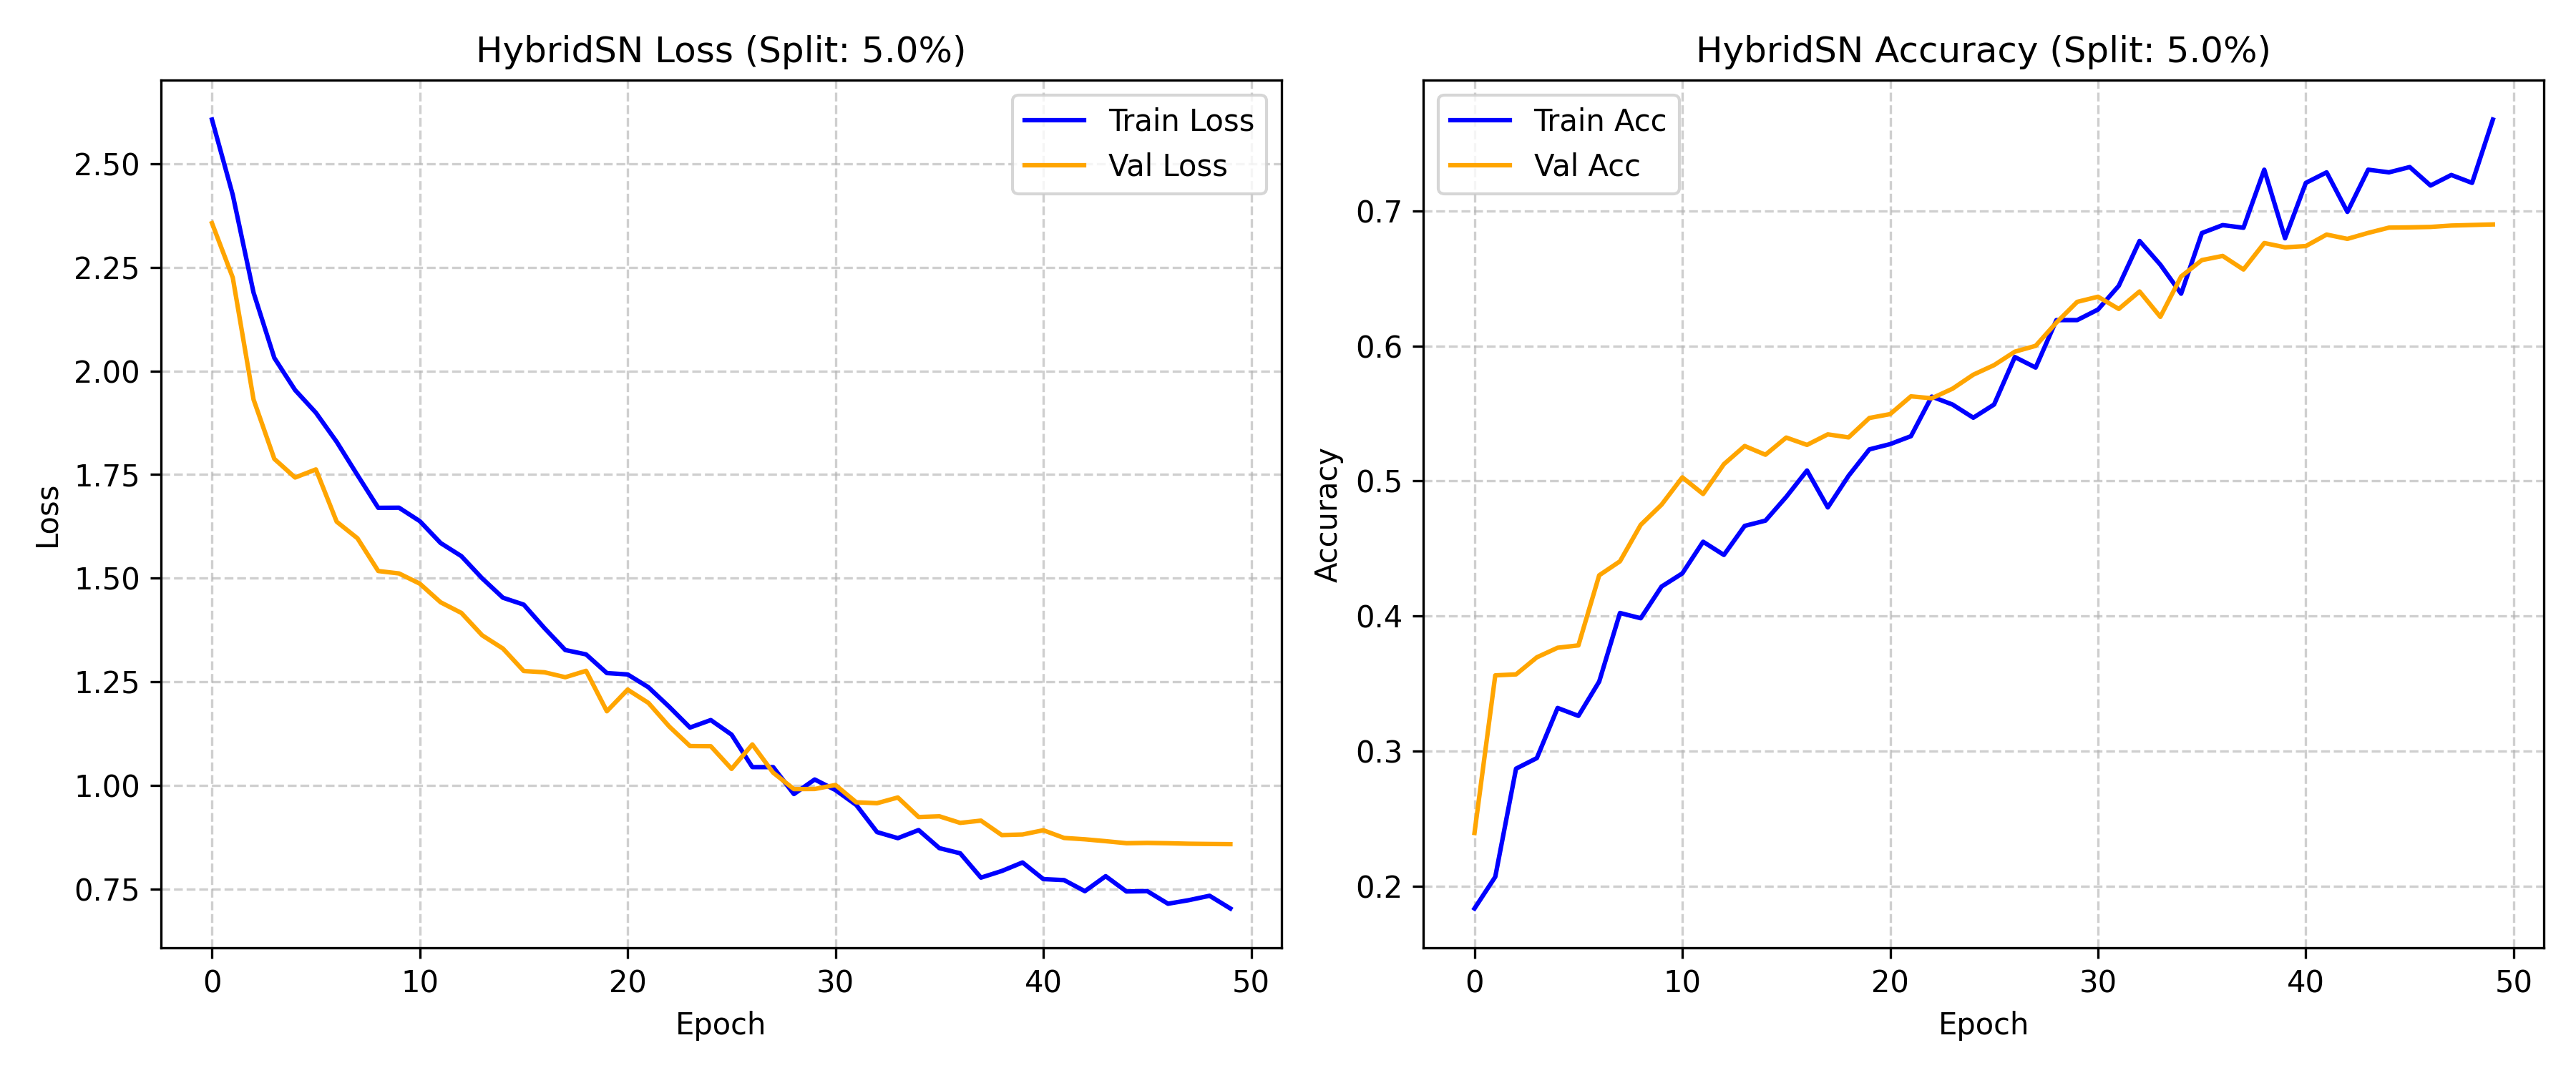
\includegraphics[width=0.48\textwidth]{Figure_Training_Curves_HybridSN_5pct.png}
    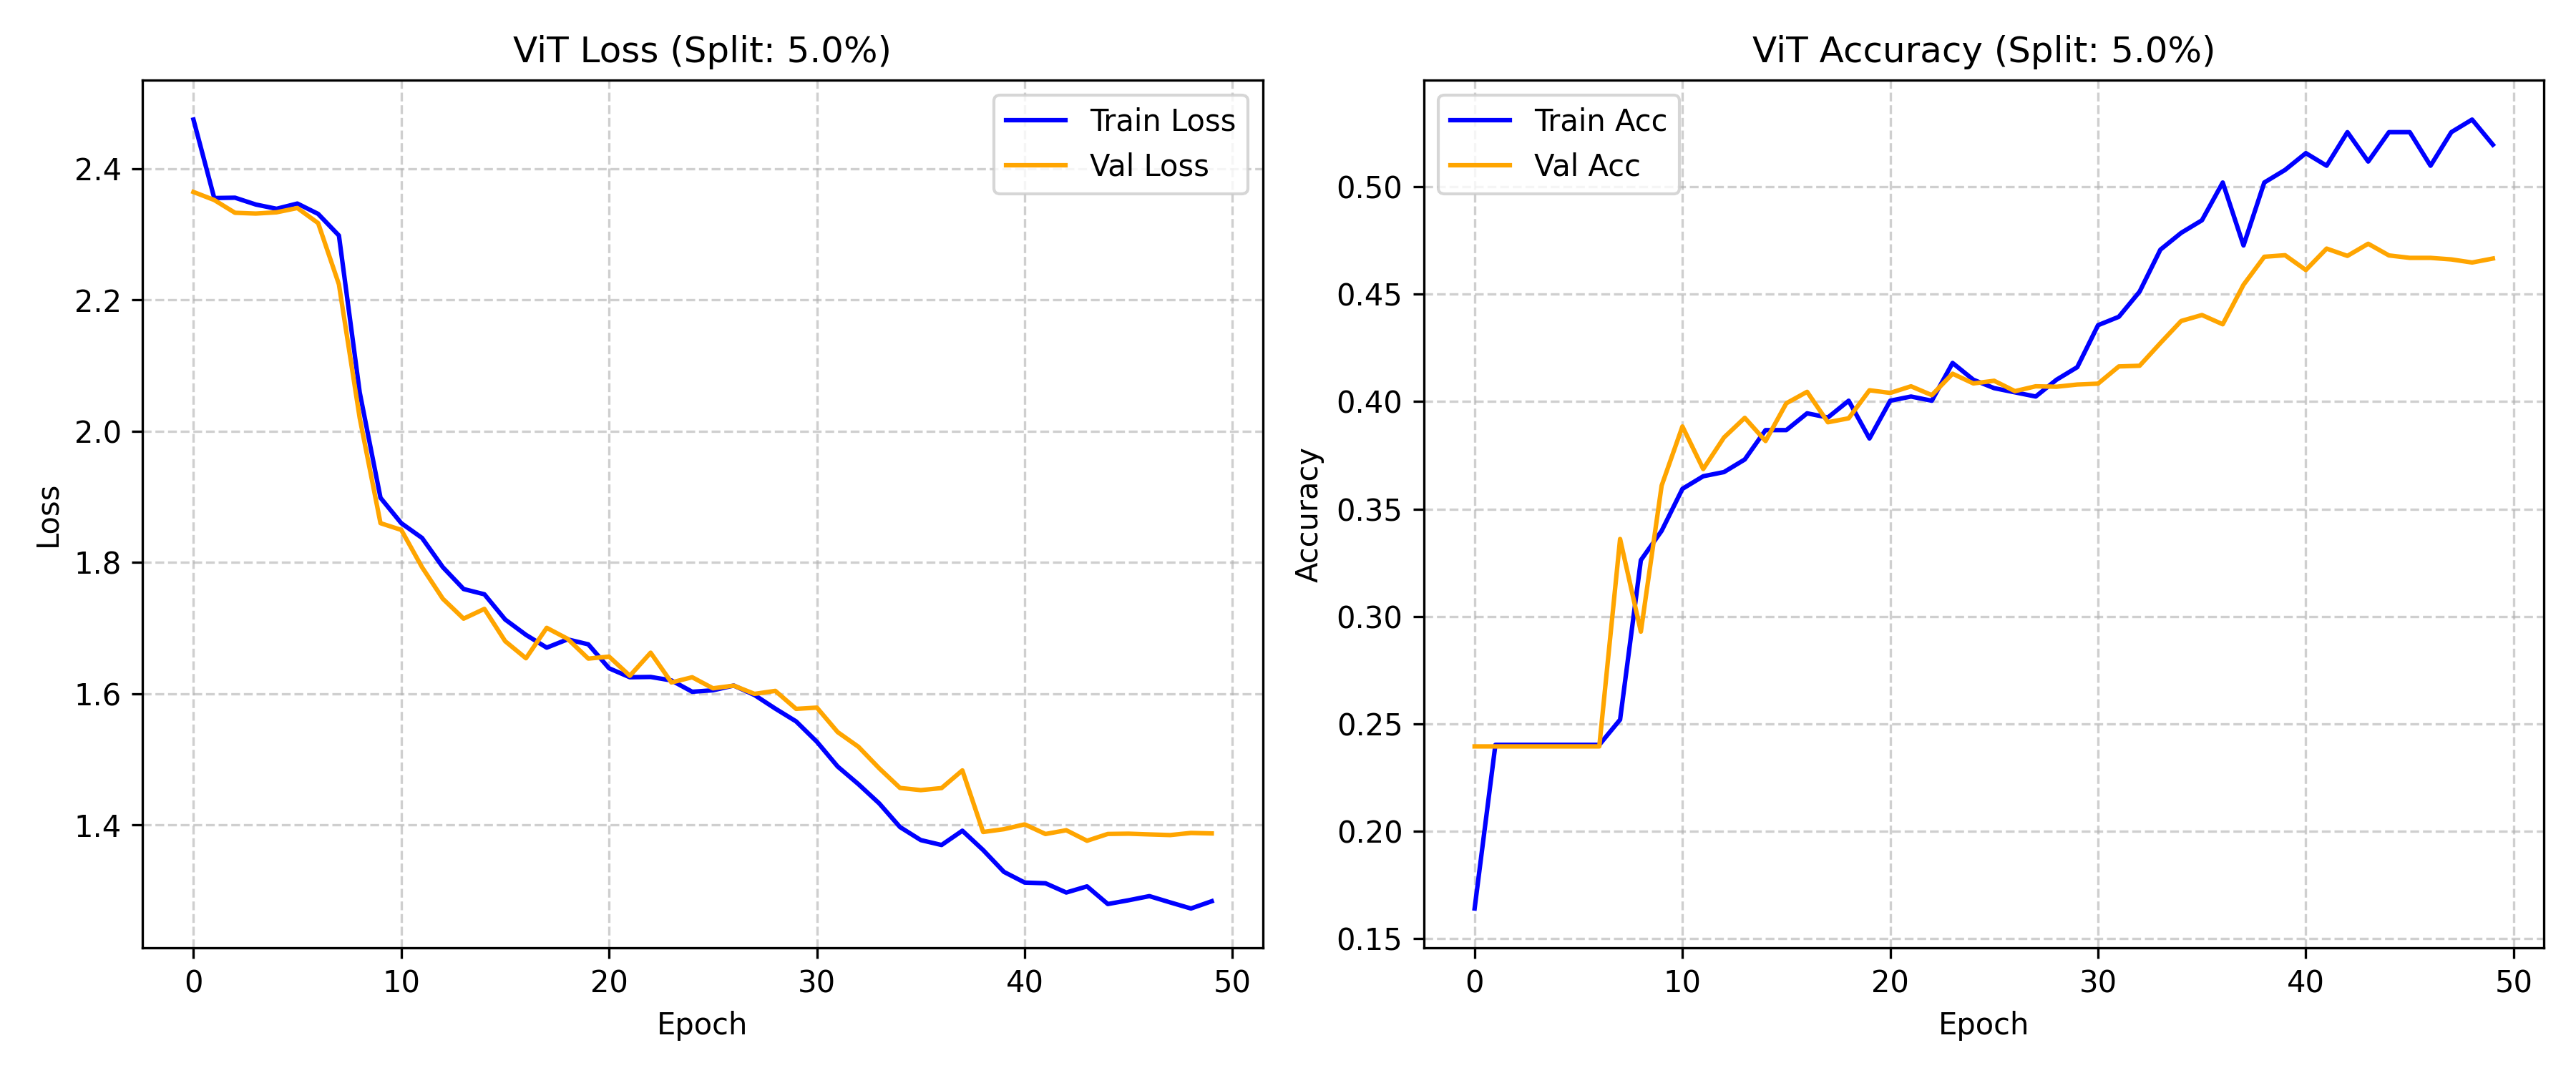
\includegraphics[width=0.48\textwidth]{Figure_Training_Curves_ViT_5pct.png}\\
    \vspace{1em}
    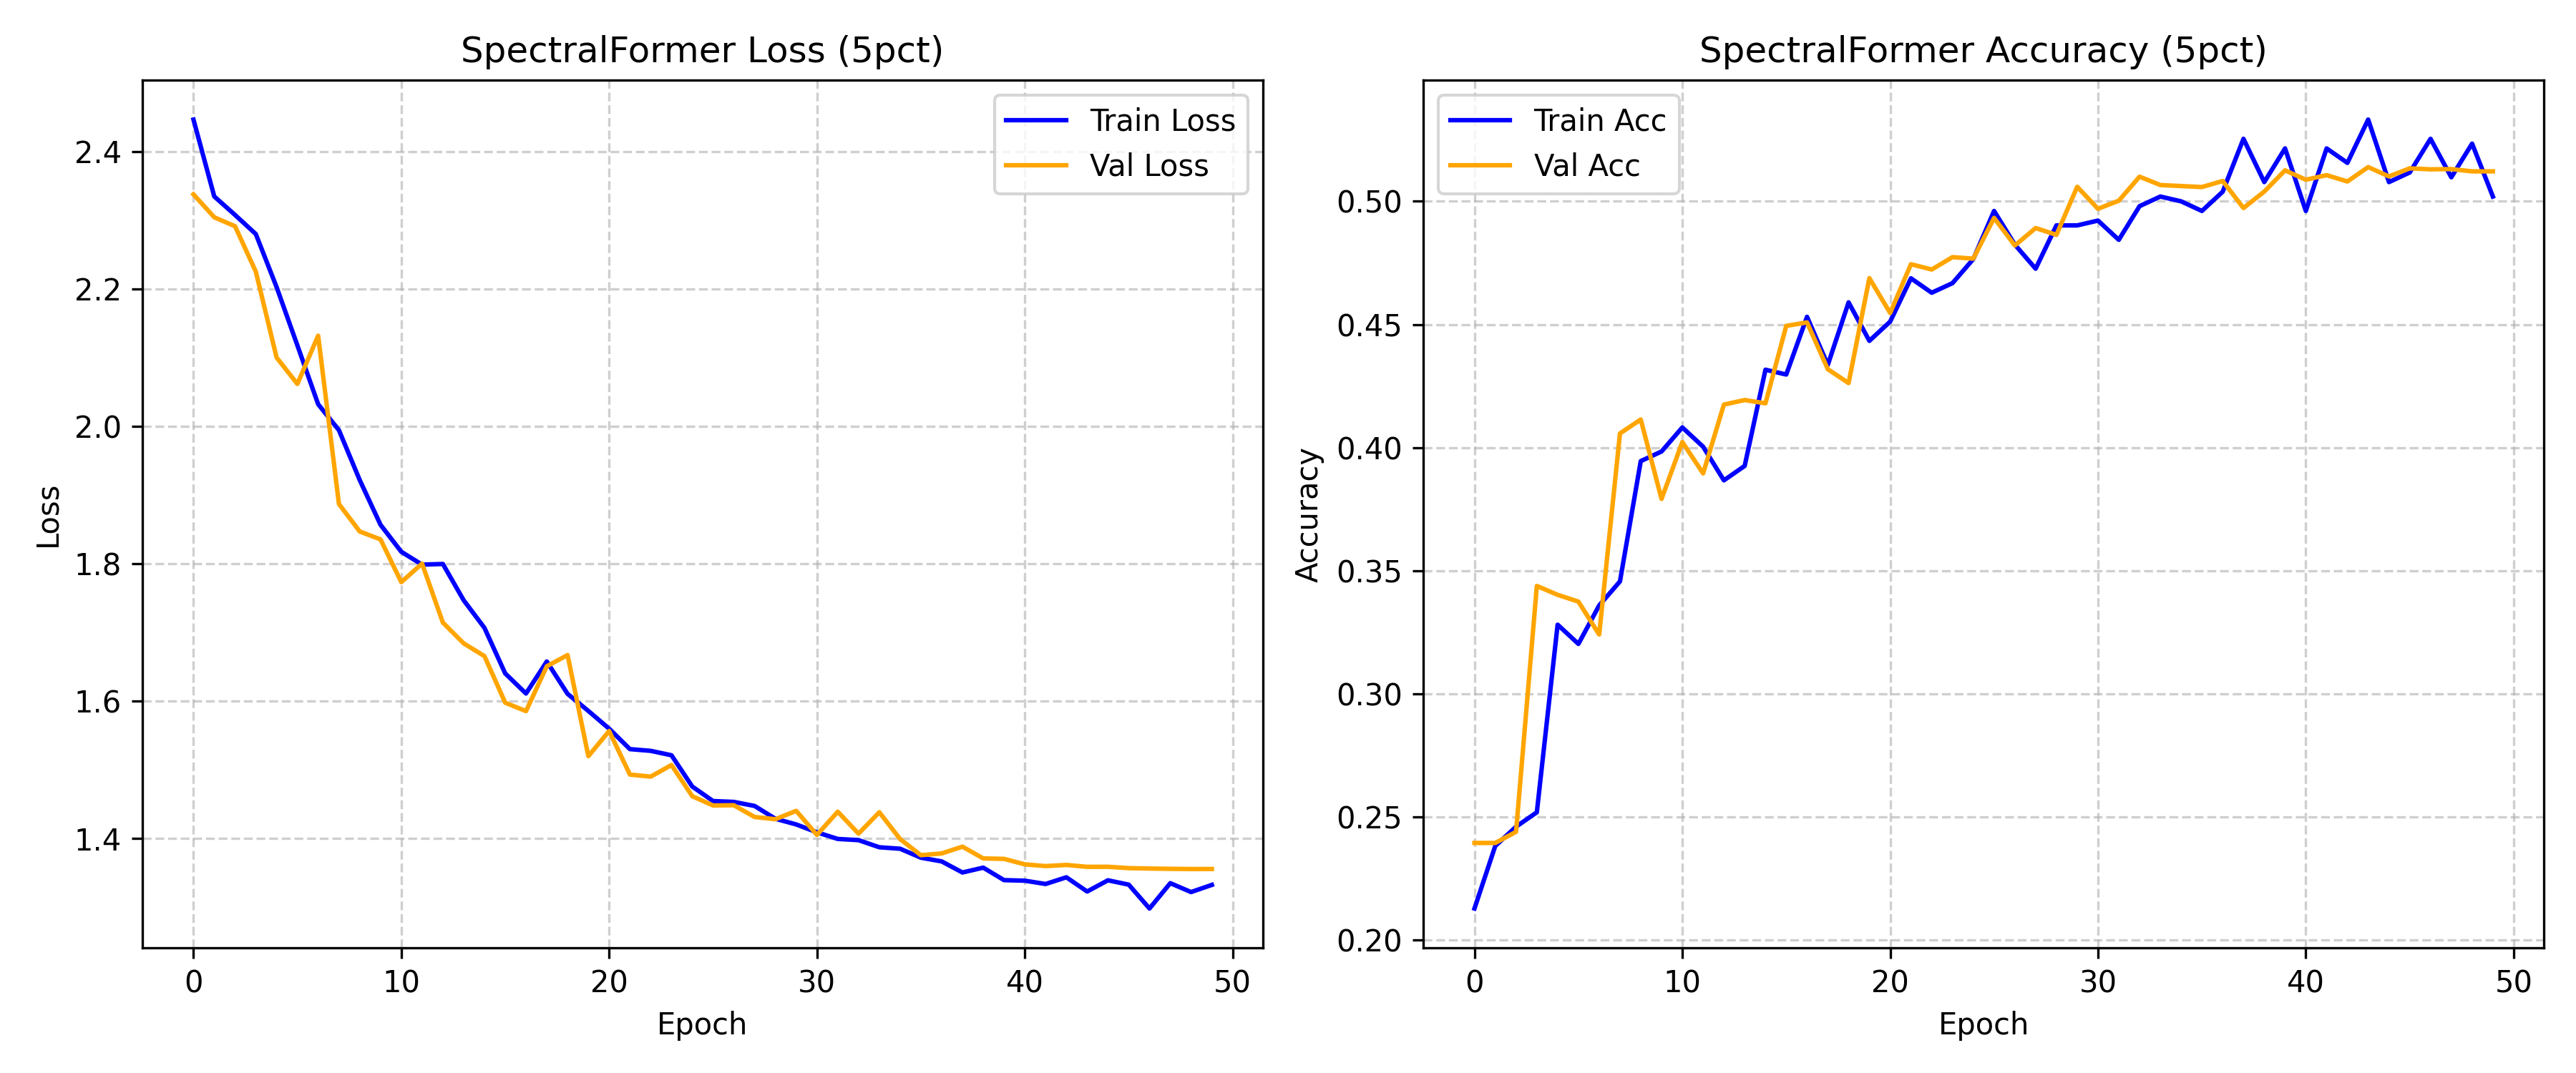
\includegraphics[width=0.48\textwidth]{Figure_Training_Curves_SpectralFormer_5pct.png}
    \caption{Representative example of training and validation loss curves for HybridSN (top-left), ViT (top-right), and SpectralFormer-inspired (bottom) at the 5\% split. HybridSN converges robustly, while both Transformers exhibit extreme overfitting, suggesting that these heavily parameterized sequence models are highly susceptible to severe overfitting on small-scale spectral datasets.}
    \label{fig:training_curves}
\end{figure*}
\subsection{Ablation Analysis: Deconstructing Data Starvation}
To systematically isolate the failure modes of deep sequence models and answer critical architectural questions, we conducted a rigorous four-part ablation study. All ablations share an identical training pipeline (optimizer, scheduler, early stopping) and utilize robust 5-seed confidence intervals to guarantee scientific validity.

\subsubsection{Ablation 1: Capacity Scaling (Depth)}
A natural hypothesis for the ViT's failure under data starvation is excessive model capacity. To investigate whether the ViT is simply ``too deep'' for the dataset, we scaled the number of transformer layers across $d \in \{1, 2, 4, 8\}$. 

\begin{figure}[h]
    \centering
    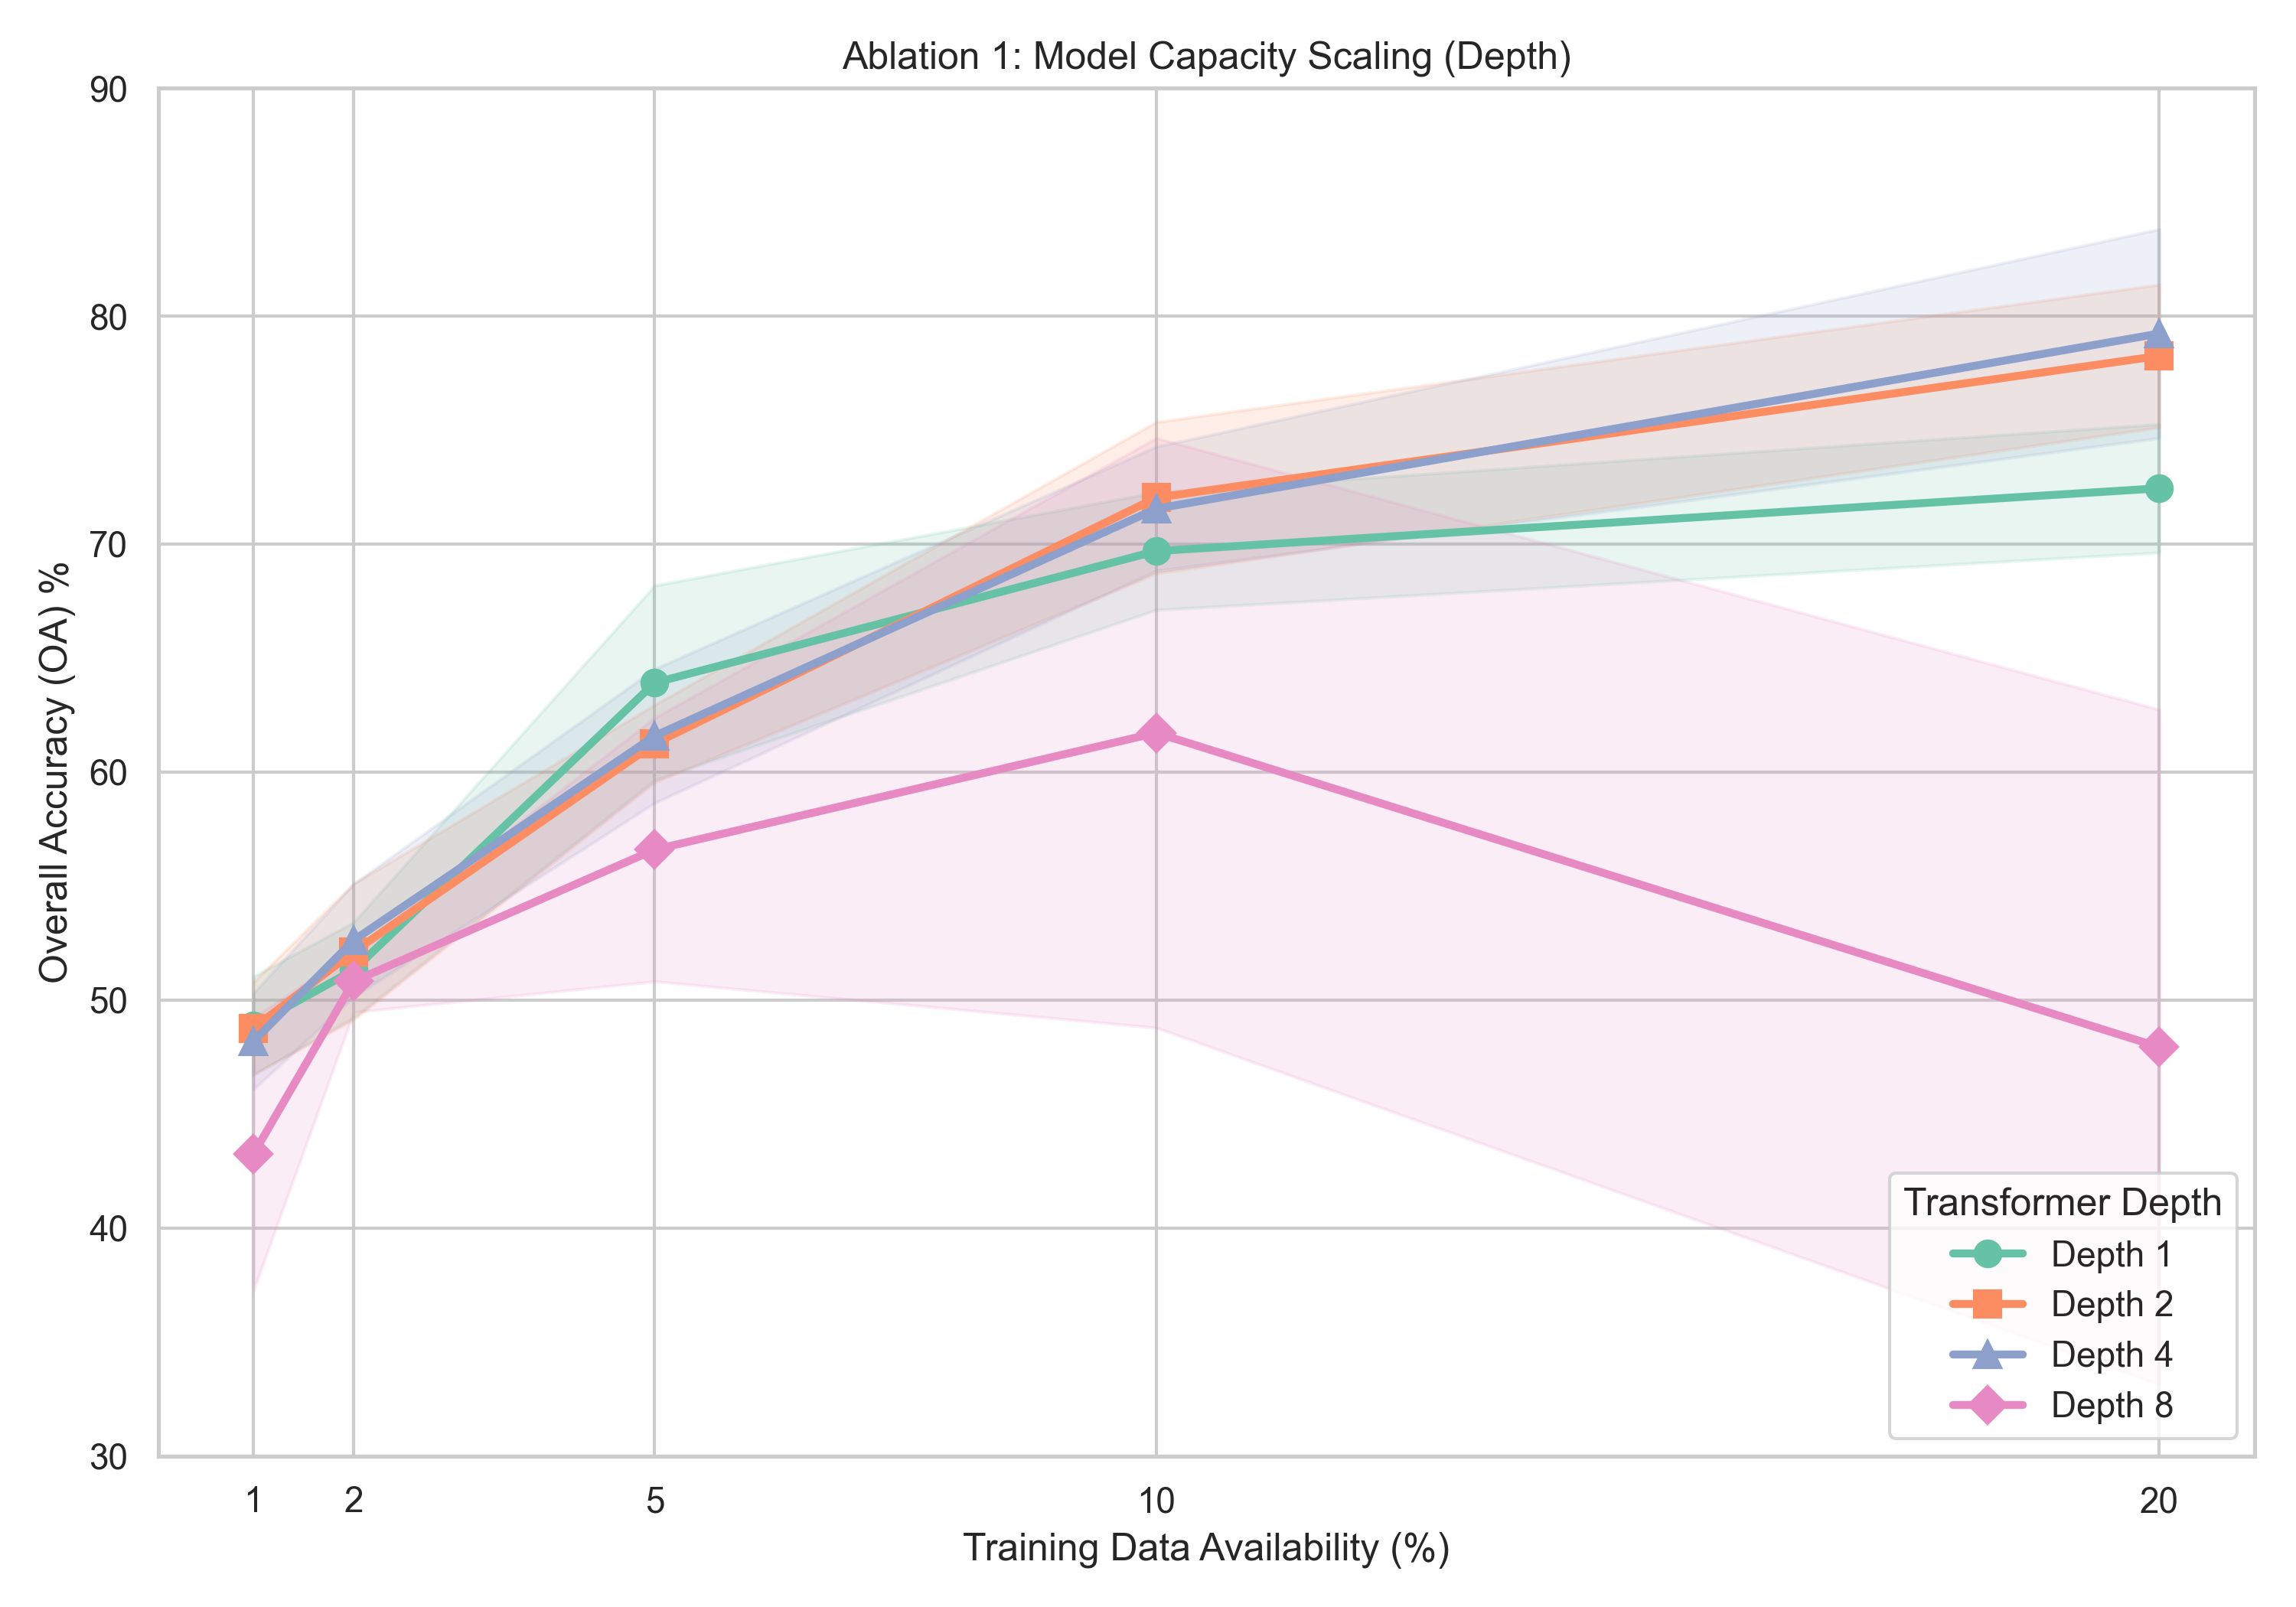
\includegraphics[width=\columnwidth]{Figure_Ablation_Depth.png}
    \caption{Ablation 1: Model Capacity Scaling (Depth) on Indian Pines. Excessive capacity ($d=8$) collapses, while shallower models ($d \in \{1, 2\}$) demonstrate resilience at extreme 1-2\% starvation splits.}
    \label{fig:ablation_depth}
\end{figure}

As depicted in Figure \ref{fig:ablation_depth}, high parameter capacity (Depth 8) leads to severe instability, culminating in mode collapse and high variance at higher splits ($47.93\% \pm 10.67$ at 20\% split). Conversely, shallower models ($d=1$ and $d=2$) act as stronger regularizers, outperforming Depth 4 in the extreme 1\% to 2\% regimes. Crucially, although shallower models showed improved stability, the Friedman statistical test across all depths at the 5\% split indicated that the performance differences were not statistically significant ($p=0.0624$). Reducing capacity delays catastrophic overfitting but does not fundamentally resolve the data-efficiency gap.

\subsubsection{Ablation 2: Attention Complexity (Heads)}
We next investigated if multi-head complexity is the primary bottleneck. Altering the number of attention heads across $h \in \{1, 2, 4, 8\}$ (while keeping embedding dimensionality constant) produced negligible variance. For instance, at the 10\% split, mean accuracy remained tightly bounded between $72.04\%$ and $73.11\%$ across all configurations. Computational overhead (inference time) remained nearly identical. This plateau occurs because increasing the number of attention heads divides the fixed representation capacity of the model rather than increasing its overall effective capacity. In a severely data-starved environment, partitioning the projection space into smaller, narrower sub-spaces fails to provide any meaningful representational advantage. These results suggest that the model is robust to multi-head partitioning; the evaluated attention-based architectures remained substantially more data-hungry than CNN-based models.

\subsubsection{Ablation 3: Isolated Inductive Bias (ConvStem)}
To investigate the hypothesis that 3D convolutions extract superior localized features compared to sequence models, we mathematically matched the intermediate dimensionality bottleneck of a ConvStem ViT and a ViT. Both models receive an identical $15 \times 15$ spatial patch; however, the ViT utilizes a dense flattening layer designed to better isolate the effect of local inductive bias, mapping 225 pixels $\rightarrow$ 16 features.

\begin{figure}[h]
    \centering
    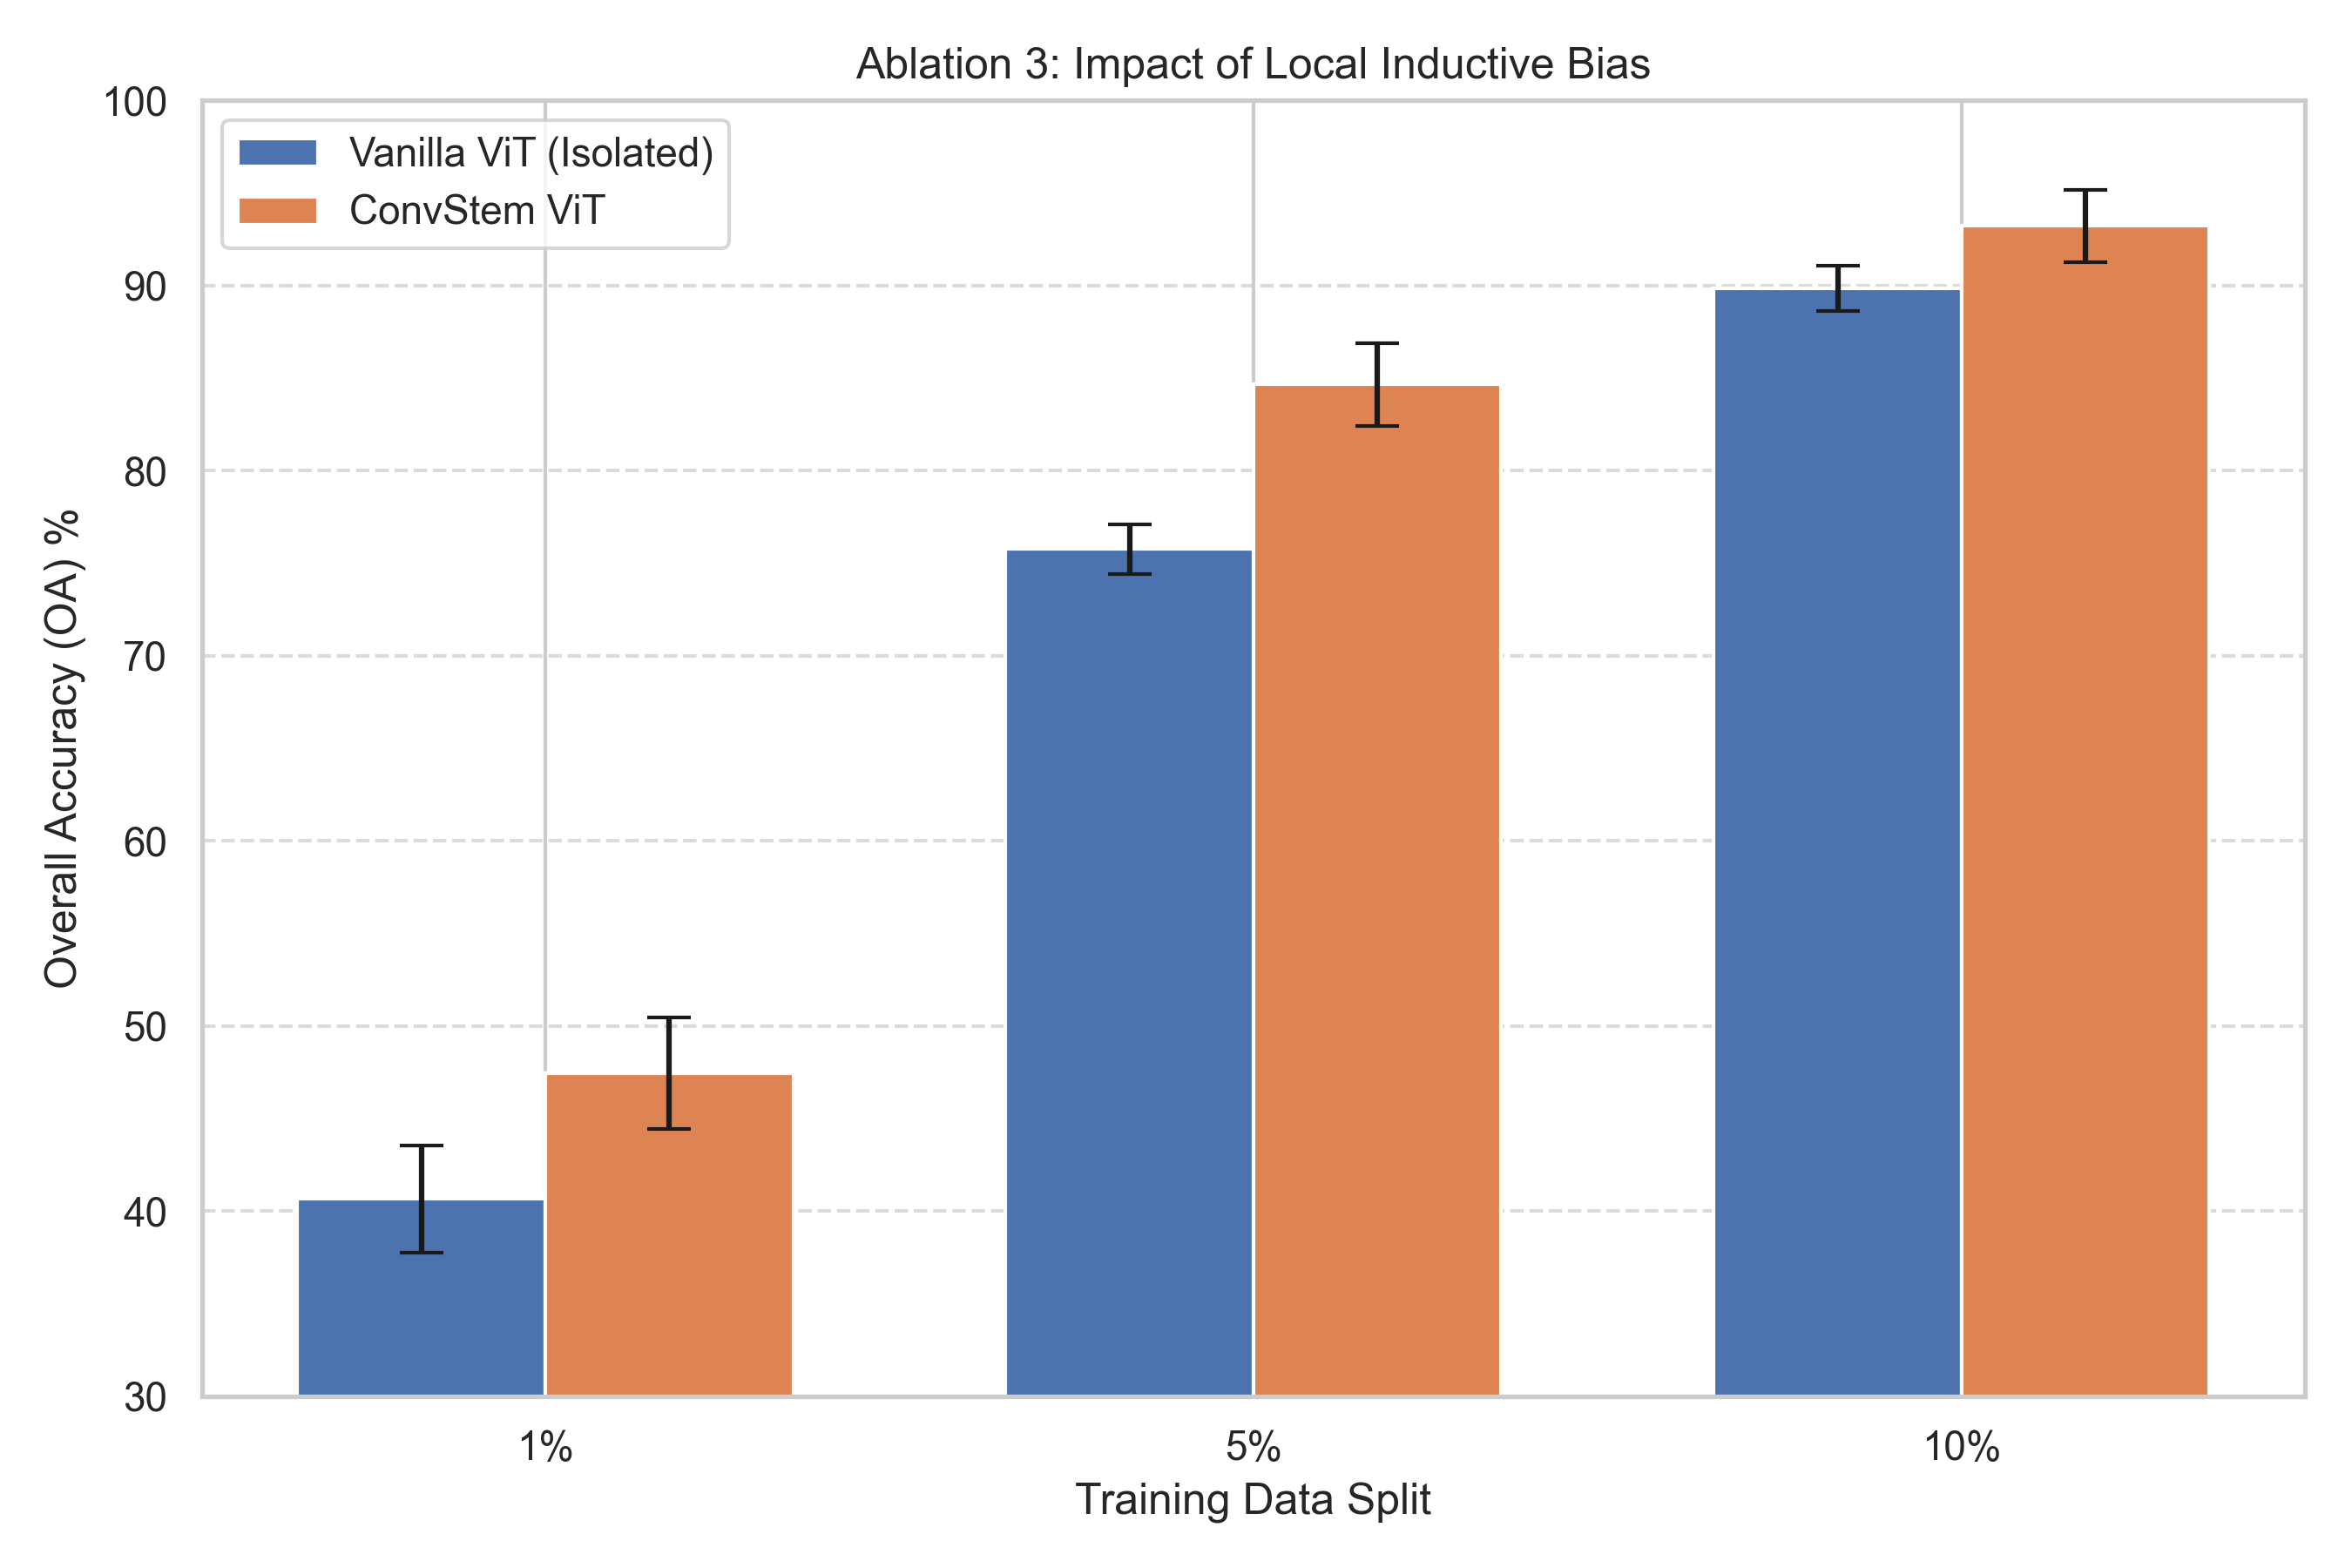
\includegraphics[width=\columnwidth]{Figure_Ablation_ConvStem.png}
    \caption{Ablation 3: Impact of Local Inductive Bias. The 3D-ConvStem consistently outperforms dense spatial flattening across all splits, suggesting the importance of local feature extraction.}
    \label{fig:ablation_convstem}
\end{figure}

As shown in Figure \ref{fig:ablation_convstem}, the ConvStem ViT consistently outperforms the isolated ViT across all splits, achieving an absolute gain of nearly 9\% ($84.65\%$ vs $75.75\%$) at the 5\% split. These results are consistent with the hypothesis that local inductive biases (3D spatial convolutions) extract significantly more robust spatial-spectral representations compared to unconstrained linear projections.

\subsubsection{Ablation 4: Linear Probe Representation Quality}
Finally, we tested the absolute quality of pre-trained representations via True Linear Probing. We froze the entire encoder backbone (locking running statistics) and trained only a linear classification head. 

\begin{figure}[h]
    \centering
    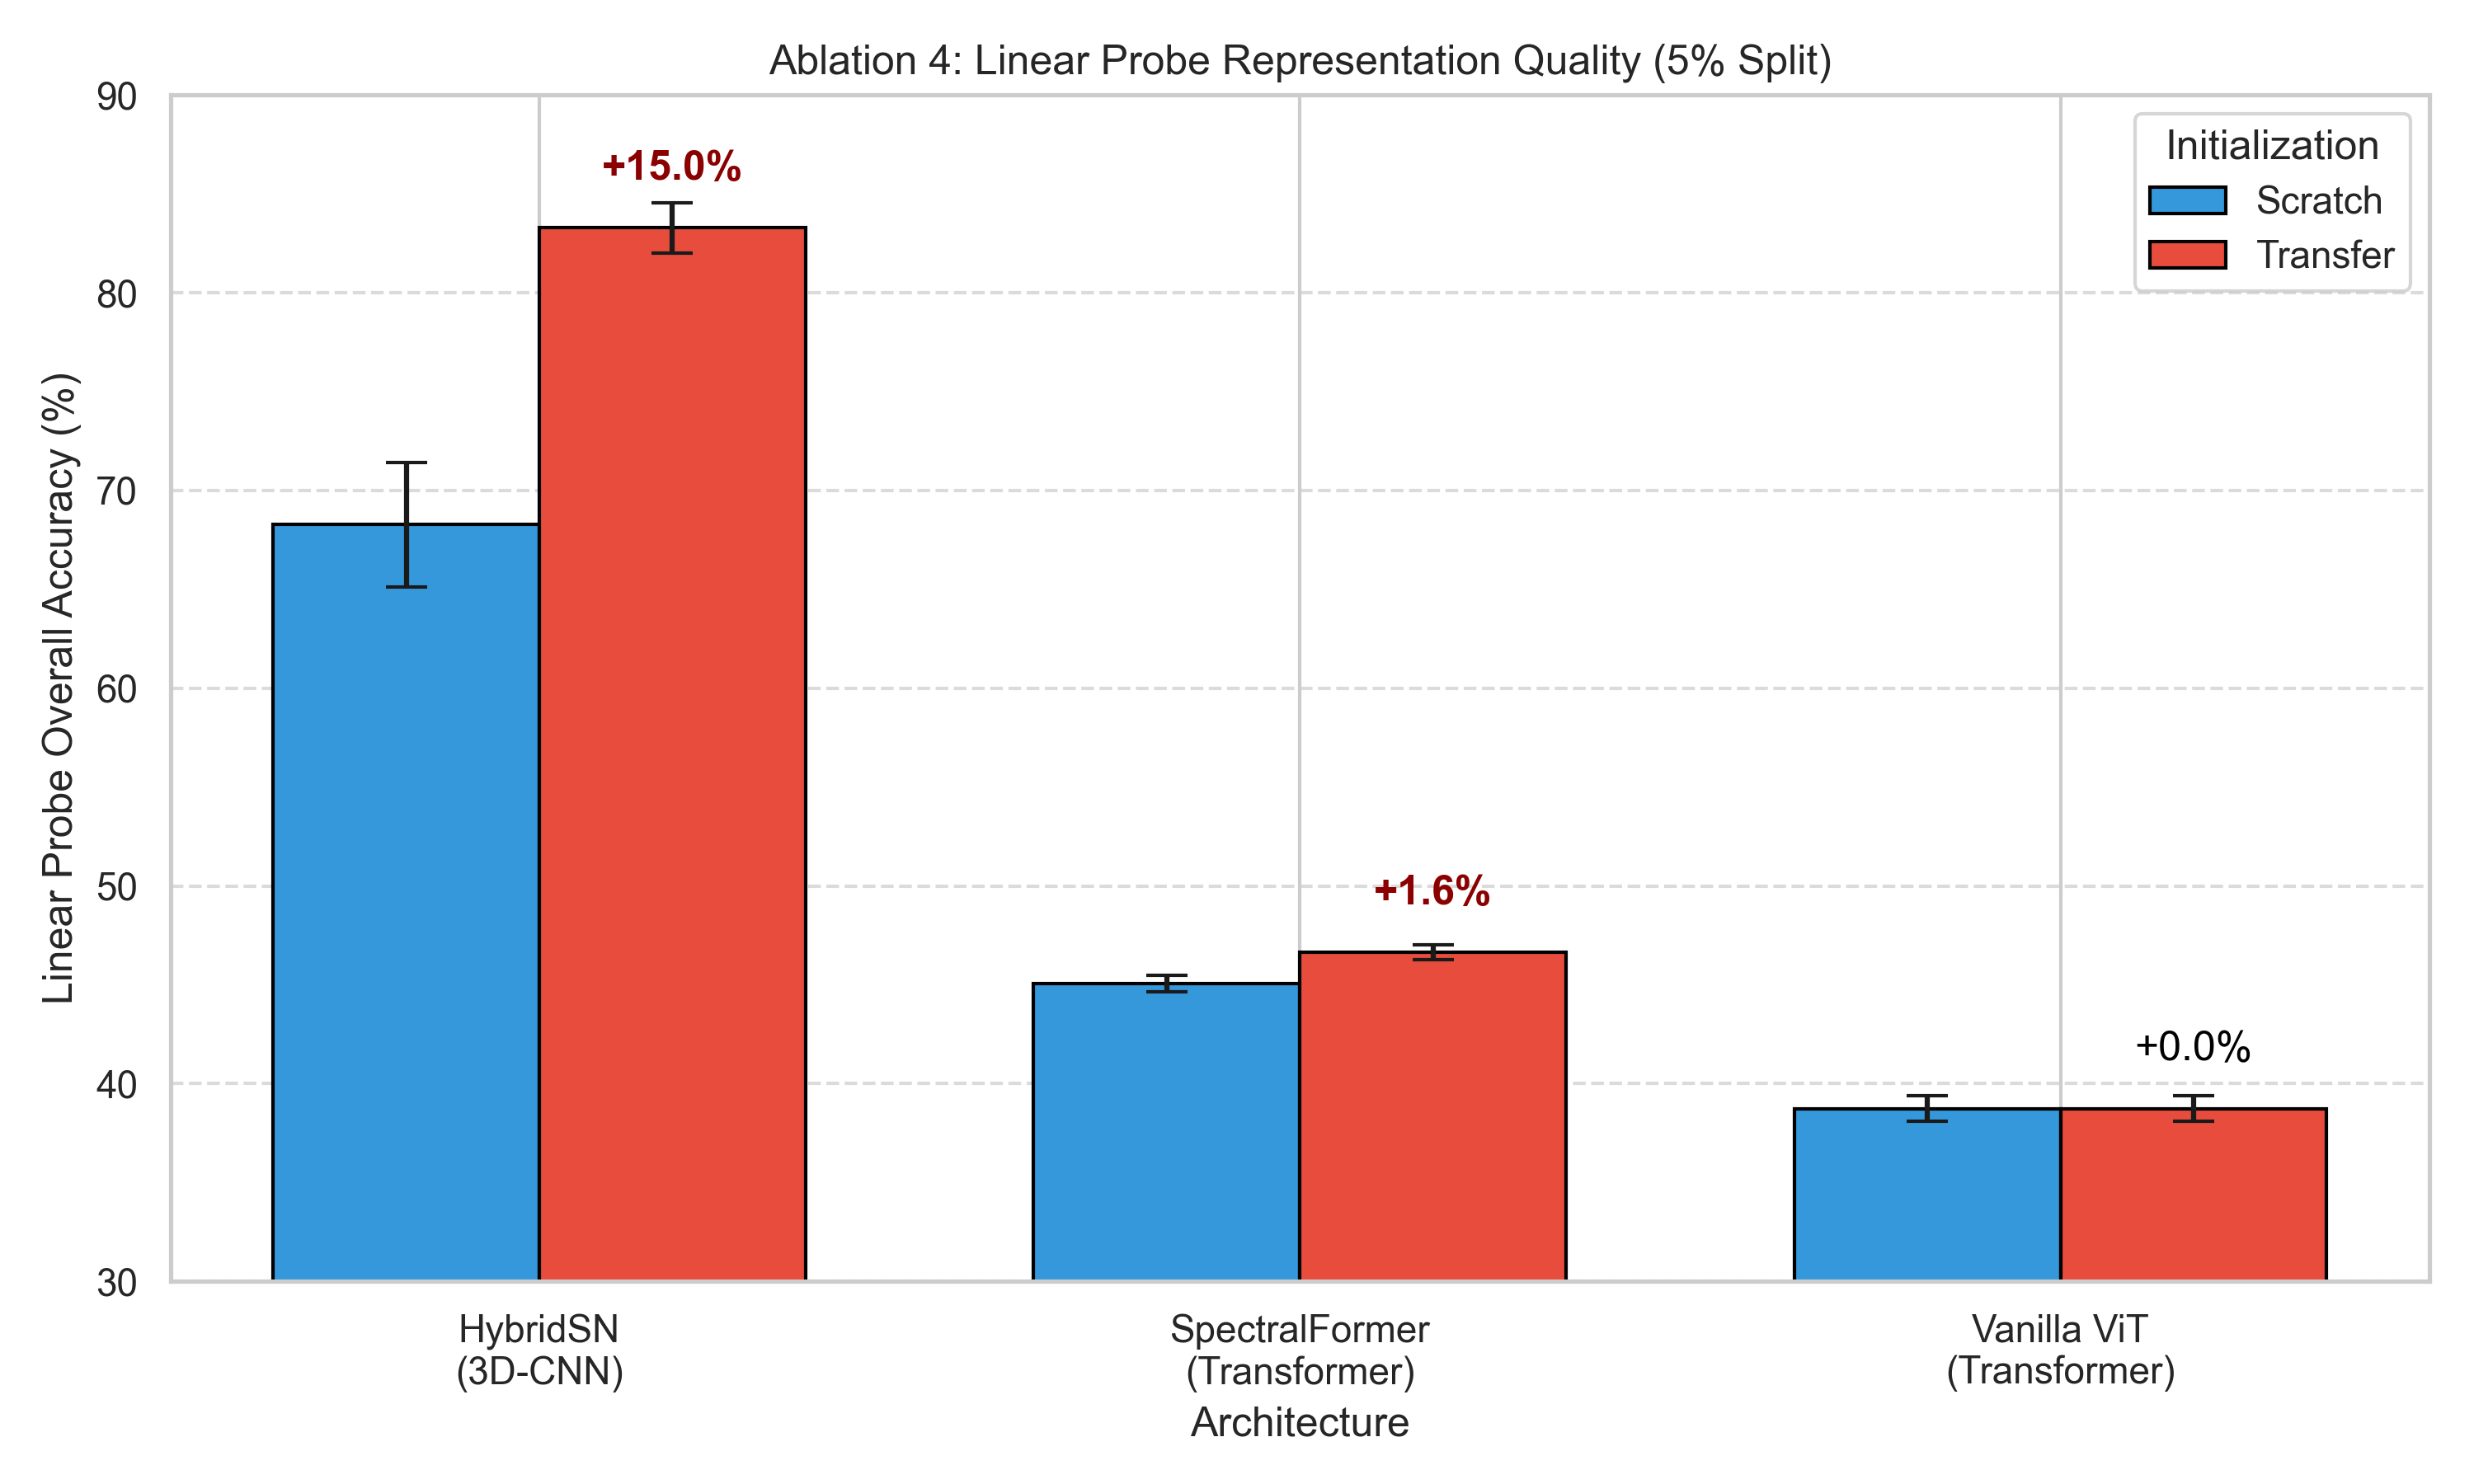
\includegraphics[width=\columnwidth]{Figure_Ablation_LinearProbe.png}
    \caption{Ablation 4: Linear Probe Classification (5\% Split). HybridSN transfers robust, linearly separable features (+15\% gain), while the evaluated transformer implementations exhibited negligible transfer gains under this annotation regime.}
    \label{fig:ablation_probe}
\end{figure}

The linear probe results (Figure \ref{fig:ablation_probe}) indicate limited transferability in Transformer transferability for HSI. When transferring from Local Soil to Indian Pines (5\% split), HybridSN achieved a substantial $+15.01\%$ gain (68.27\% $\rightarrow$ 83.28\%). In stark contrast, both ViT and SpectralFormer-inspired exhibited near-zero transfer gains ($0\%$ and $+1.58\%$, respectively). This provides evidence that while CNNs effectively learn robustly transferable spatial-texture edge filters, the evaluated transformer implementations failed to abstract linearly separable, domain-agnostic features without a large-scale pre-training initialization. Crucially, this explains why HybridSN successfully transfers while the ViT fails: the 3D-ConvStem inherently encodes strong local spatial-spectral inductive biases during pre-training. These inductive biases yield generalized, transferable feature representations that remain linearly separable in the target domain, unlike the unconstrained global representations of the evaluated pure attention models.

\subsection{Bridging the Gap via Transfer Learning}
Given the stark contrast between the abundant and data-starved regimes, we explored whether the inherent data-hunger of deep sequence architectures could be satisfied by pre-training on abundant source datasets before fine-tuning on starved target environments. We executed a rigorous multi-seed transfer protocol across two opposing domain hierarchies. 

\begin{figure*}[h]
\centering
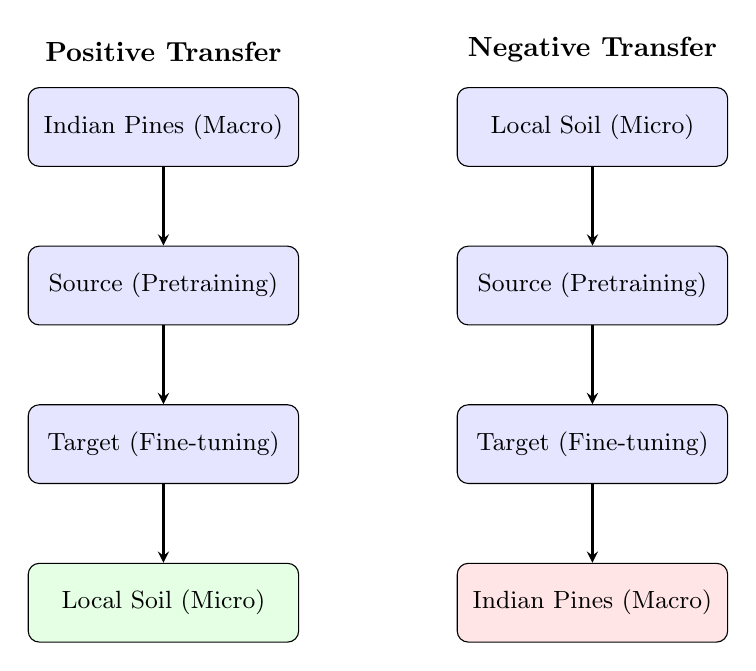
\begin{tikzpicture}[
    node distance=1.0cm,
    box/.style={draw, rectangle, rounded corners, fill=blue!10, text width=3.2cm, align=center, minimum height=1cm, font=\small},
    arrow/.style={->, >=stealth, thick}
]
% Positive transfer learning
\node[box] (ip1) {Indian Pines (Macro)};
\node[box, below=of ip1] (pre1) {Source (Pretraining)};
\node[box, below=of pre1] (fine1) {Target (Fine-tuning)};
\node[box, below=of fine1, fill=green!10] (ls1) {Local Soil (Micro)};
\draw[arrow] (ip1) -- (pre1);
\draw[arrow] (pre1) -- (fine1);
\draw[arrow] (fine1) -- (ls1);
\node[above=0.2cm of ip1, font=\bfseries] {Positive Transfer};

% Negative transfer learning
\node[box, right=2cm of ip1, fill=blue!10] (ls2) {Local Soil (Micro)};
\node[box, below=of ls2, fill=blue!10] (pre2) {Source (Pretraining)};
\node[box, below=of pre2, fill=blue!10] (fine2) {Target (Fine-tuning)};
\node[box, below=of fine2, fill=red!10] (ip2) {Indian Pines (Macro)};
\draw[arrow] (ls2) -- (pre2);
\draw[arrow] (pre2) -- (fine2);
\draw[arrow] (fine2) -- (ip2);
\node[above=0.2cm of ls2, font=\bfseries] {Negative Transfer};
\end{tikzpicture}
\caption{Bidirectional Transfer Learning framework illustrating the tested domain hierarchies.}
\label{fig:transfer_diagram}
\end{figure*}

\subsubsection{The Power of Positive Transfer (Indian Pines (Macro) $\rightarrow$ Local Soil (Micro))}
In our first scenario, we evaluated transferring from the public Indian Pines AVIRIS dataset (abundant source) to our Local UAV Soil dataset (starved target). Despite the Indian Pines dataset capturing macro-level agricultural canopies and the Local dataset capturing micro-level soil textures, the high-altitude spectral diversity of Indian Pines acted as a strong foundational prior.

\begin{table*}[t]
\centering
\caption{Cross-Domain Transfer Learning: Indian Pines (Macro) $\rightarrow$ Local Soil (Micro)}\label{tab:transfer_ip_to_local}
\resizebox{\textwidth}{!}{
\begin{tabular}{lccccc}
\toprule
\textbf{Model} & \textbf{Data Split} & \textbf{Scratch OA (\%)} & \textbf{Transfer OA (\%)} & \textbf{Abs. Gain (\%)} & \textbf{Rel. Gain (\%)} \\
\midrule
ViT & 1\% & $35.12 \pm 6.61$ & $71.92 \pm 5.08$ & \textbf{+36.80} & \textbf{+104.78} \\
ViT & 5\% & $42.14 \pm 13.33$ & $82.17 \pm 1.71$ & \textbf{+40.03} & \textbf{+94.99} \\
ViT & 10\% & $38.78 \pm 12.74$ & $85.98 \pm 0.81$ & \textbf{+47.20} & \textbf{+121.71} \\
ViT & 20\% & $33.17 \pm 12.01$ & $88.81 \pm 0.71$ & \textbf{+55.64} & \textbf{+167.74} \\
\midrule
SpectralFormer-inspired & 1\% & $37.25 \pm 10.91$ & $61.03 \pm 8.60$ & \textbf{+23.78} & \textbf{+63.84} \\
SpectralFormer-inspired & 5\% & $75.87 \pm 4.31$ & $80.84 \pm 2.78$ & +4.96 & +6.55 \\
SpectralFormer-inspired & 10\% & $78.69 \pm 6.02$ & $84.57 \pm 1.37$ & +5.89 & +7.47 \\
SpectralFormer-inspired & 20\% & $84.91 \pm 4.08$ & $86.81 \pm 0.74$ & +1.90 & +2.24 \\
\midrule
HybridSN & 1\% & $46.65 \pm 14.75$ & $46.92 \pm 15.74$ & +0.27 & +0.58 \\
HybridSN & 5\% & $82.61 \pm 7.43$ & $86.10 \pm 2.65$ & \textbf{+3.49} & \textbf{+4.22} \\
HybridSN & 10\% & $87.15 \pm 17.51$ & $89.94 \pm 4.11$ & +2.79 & +3.20 \\
HybridSN & 20\% & $88.76 \pm 11.84$ & $96.82 \pm 0.43$ & \textbf{+8.06} & \textbf{+9.08} \\
\bottomrule
\end{tabular}
}
\end{table*}

As detailed in Table \ref{tab:transfer_ip_to_local} (class-wise metrics in Appendix \ref{sec:appendix}), the ViT exhibited a substantial improvement. Trained from scratch on the 1\% split, the ViT entirely failed to converge (35.12\%). However, when initialized with Indian Pines pre-trained weights, the exact same architecture achieved 71.92\% (an absolute gain of +36.80\%). At the 20\% split, the transfer gain exceeded +55\%. Except for pretrained initialization, all optimization settings were identical between scratch and transfer models. This strongly suggests that the evaluated transformer architectures are robust feature extractors in HSI, provided their self-attention matrices are initialized via hierarchical pre-training.

Furthermore, this Positive transfer learning substantially shifted the Machine Learning crossover point. Trained from scratch, the 3D-CNN (HybridSN) only surpassed the LightGBM baseline when provided with $\sim$6.6\% of the dataset. With Transfer Learning, the HybridSN crossed over at a mere 4.25\% data availability (note that these exact crossover thresholds were estimated using piecewise linear interpolation between the empirically evaluated discrete data splits). These crossover points are interpolation estimates rather than directly observed training splits. By transferring foundational spectral representations, deep learning can effectively bridge the low-resource gap and beat classical tree-based ensembles even earlier.

\subsubsection{The Domain Gap and Negative Transfer (Local Soil (Micro) $\rightarrow$ Indian Pines (Macro))}
To test the symmetry of this phenomenon, we reversed the domain hierarchy, attempting to pre-train on the Local UAV Soil dataset and fine-tune on the Indian Pines dataset. Our results revealed a severe instance of \textit{Negative transfer learning}. 

\par While the ViT trained from scratch on Indian Pines achieved 53.92\%, the ViT pre-trained on Local Soil and fine-tuned on Indian Pines collapsed to 35.90\%. The spatial-spectral domain gap between low-altitude, high-resolution uniform soil textures (UAV) and high-altitude, highly heterogeneous vegetation canopies (AVIRIS satellite) proved severe domain mismatch. The deep architectures became highly specialized to local soil micro-textures during pre-training, trapping the optimizers in local minima when suddenly confronted with macro-agriculture data. These results suggest a critical Asymmetric Cross-Domain Transfer in remote sensing: foundational pre-training only substantially improves data-starved models if the source domain hierarchically encompasses the spectral complexity of the target domain. Without explicit, complex domain adaptation techniques, raw pre-training actively harms generalization in our experiments rather than aiding it, further solidifying the appeal of off-the-shelf classical algorithms for isolated, small-scale datasets.

\subsection{SHAP Analysis}
A critical requirement for deploying HSI models in precision agriculture is ensuring they base decisions on physical realities, not dataset bias \cite{b35}. Following recent trends in remote sensing interpretability \cite{b21, b22}, our Explainable AI (SHAP) \cite{b25} analysis visually unpacks the logic of the LightGBM models across both data regimes. 

As seen in Figure \ref{fig:shap_local}, the model heavily prioritizes Band 96, 156, and 97. These bands correspond approximately to spectral regions commonly associated with specific physical properties: regions near 900-1000 nm (often corresponding to Band 96/97) are generally correlated with water and moisture absorption features, while bands further into the Short-Wave Infrared (SWIR) region (like Band 156) are typically indicative of structural soil composition, clay content, and organic matter. This is consistent with physically meaningful spectral regions reported in previous studies, suggesting resilience against spurious dataset-specific noise.

\begin{figure}[h]
    \centering
    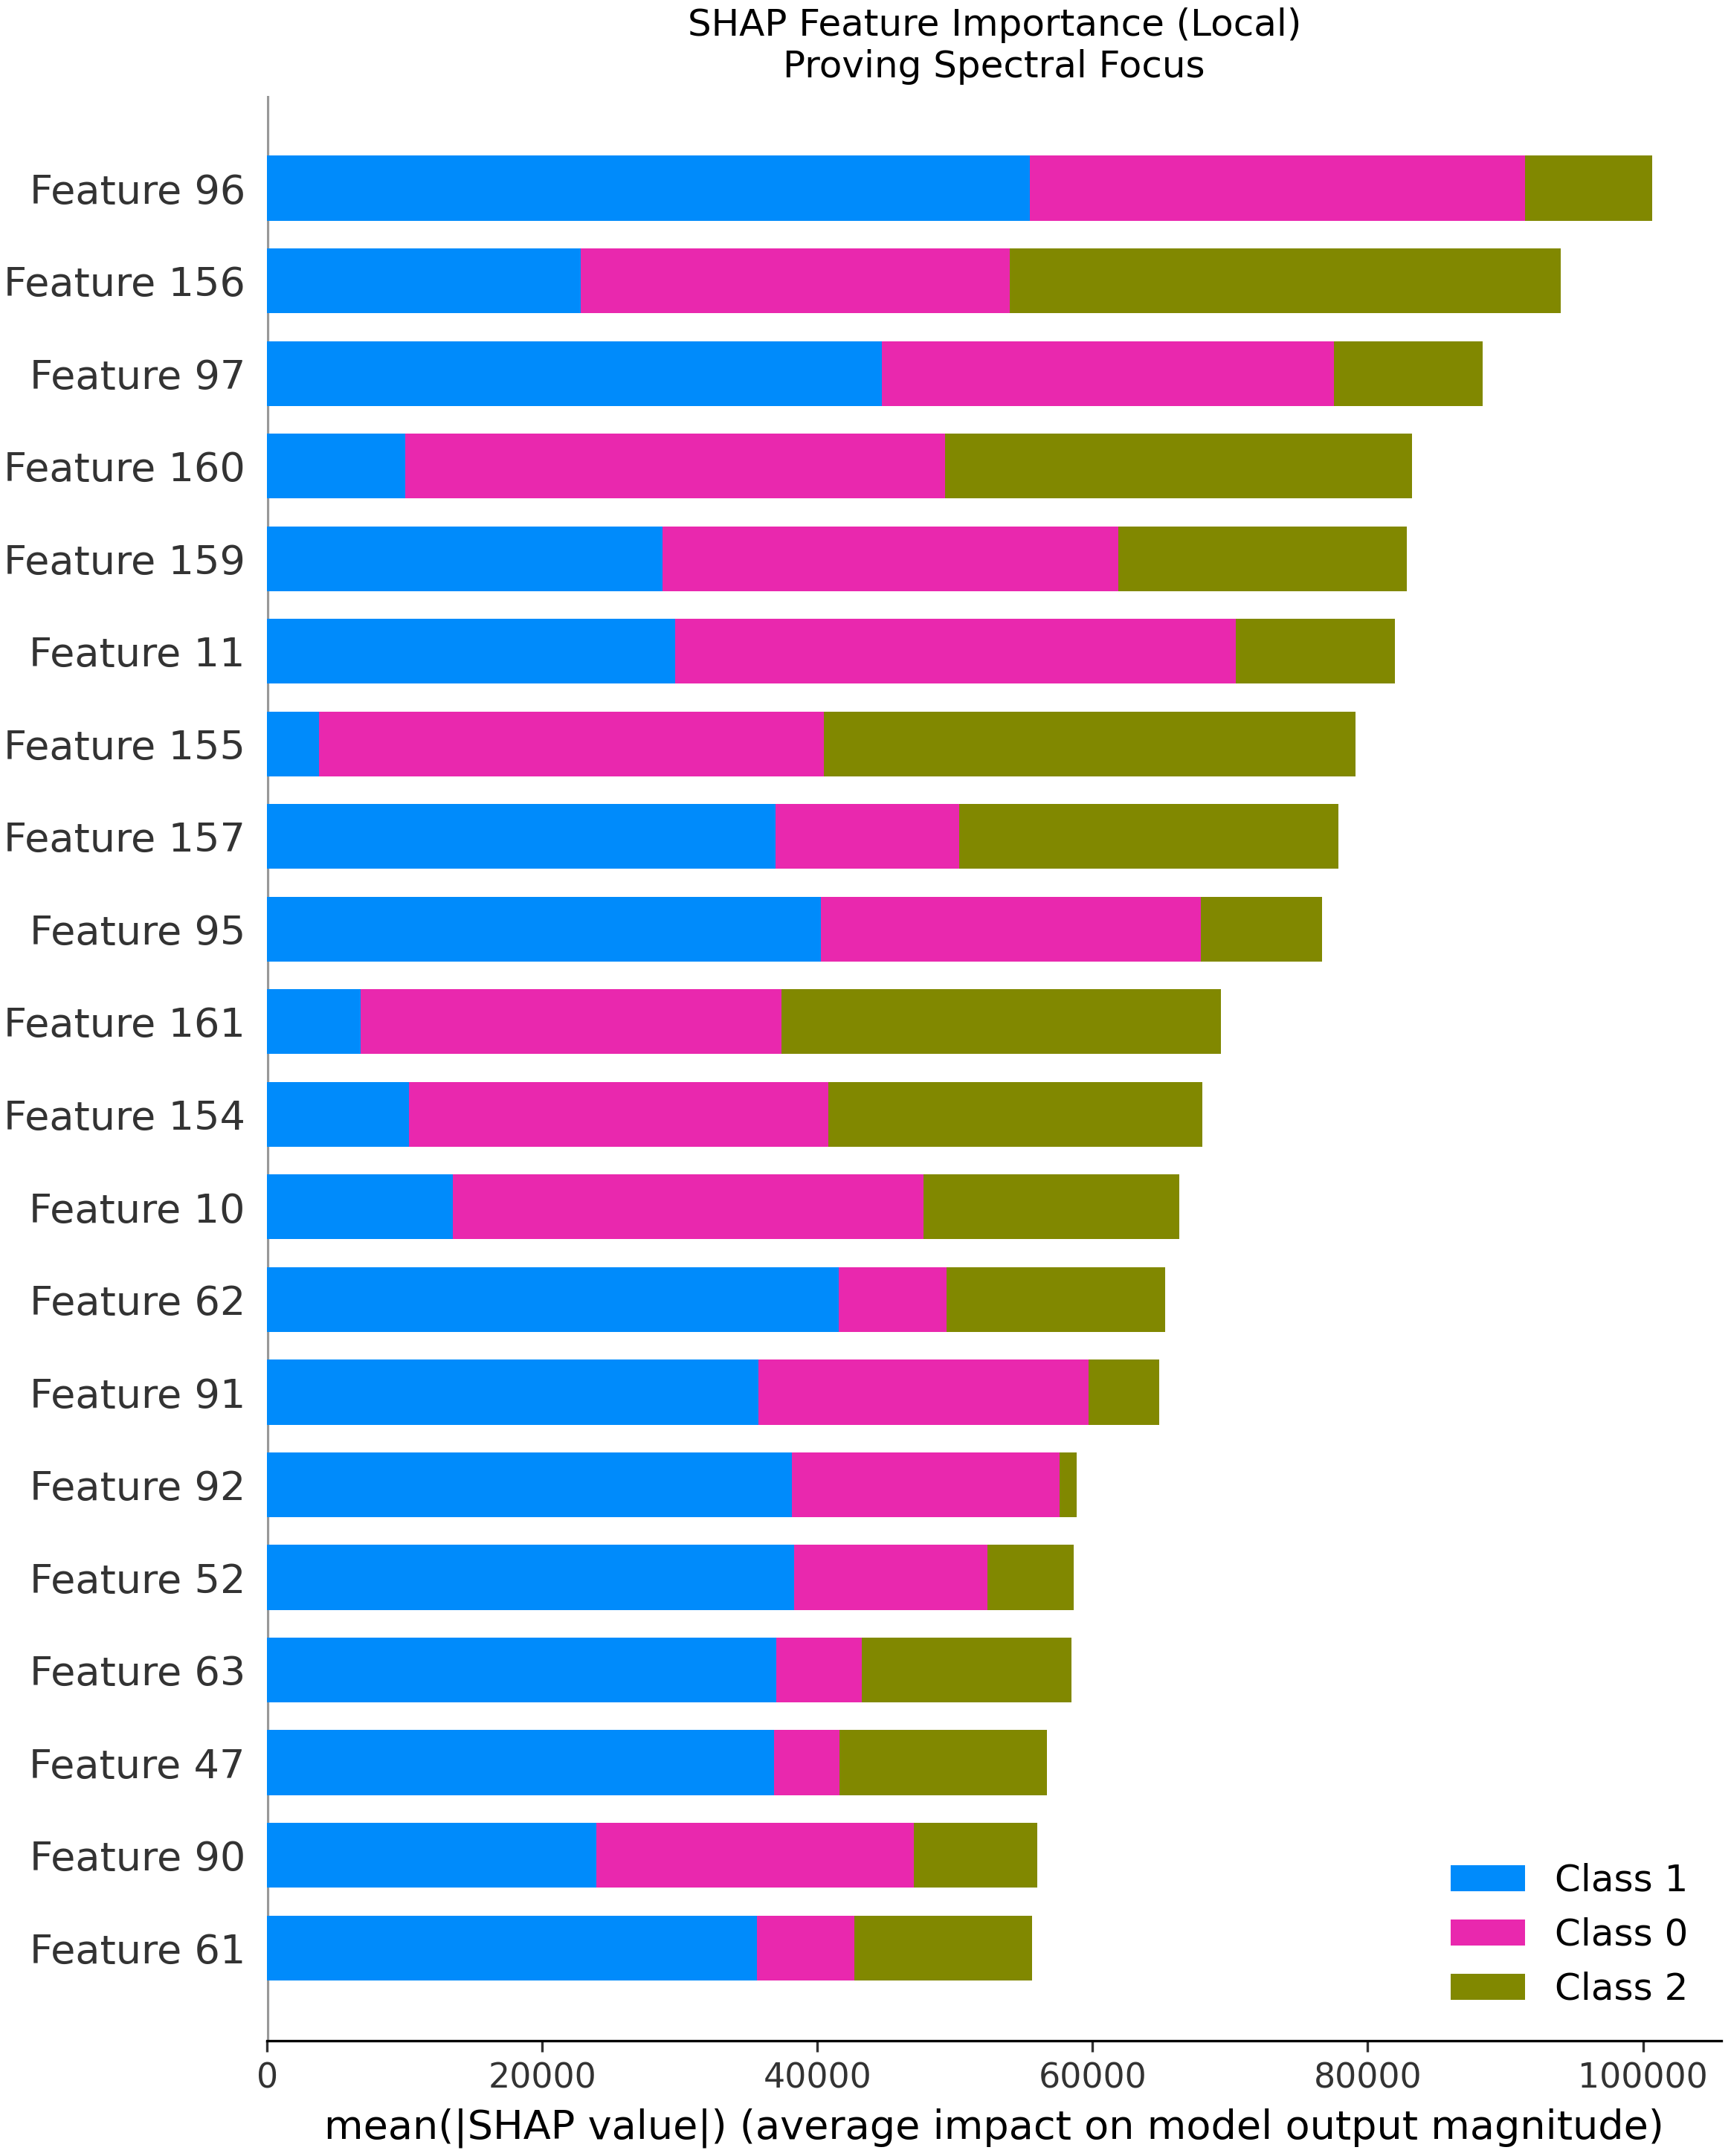
\includegraphics[width=0.48\textwidth]{Figure2_Local_SHAP_Importance.png}
    \caption{Local Soil Dataset SHAP Feature Importance, prioritizing Bands 96, 156, and 97.}
    \label{fig:shap_local}
\end{figure}

\begin{figure}[h]
    \centering
    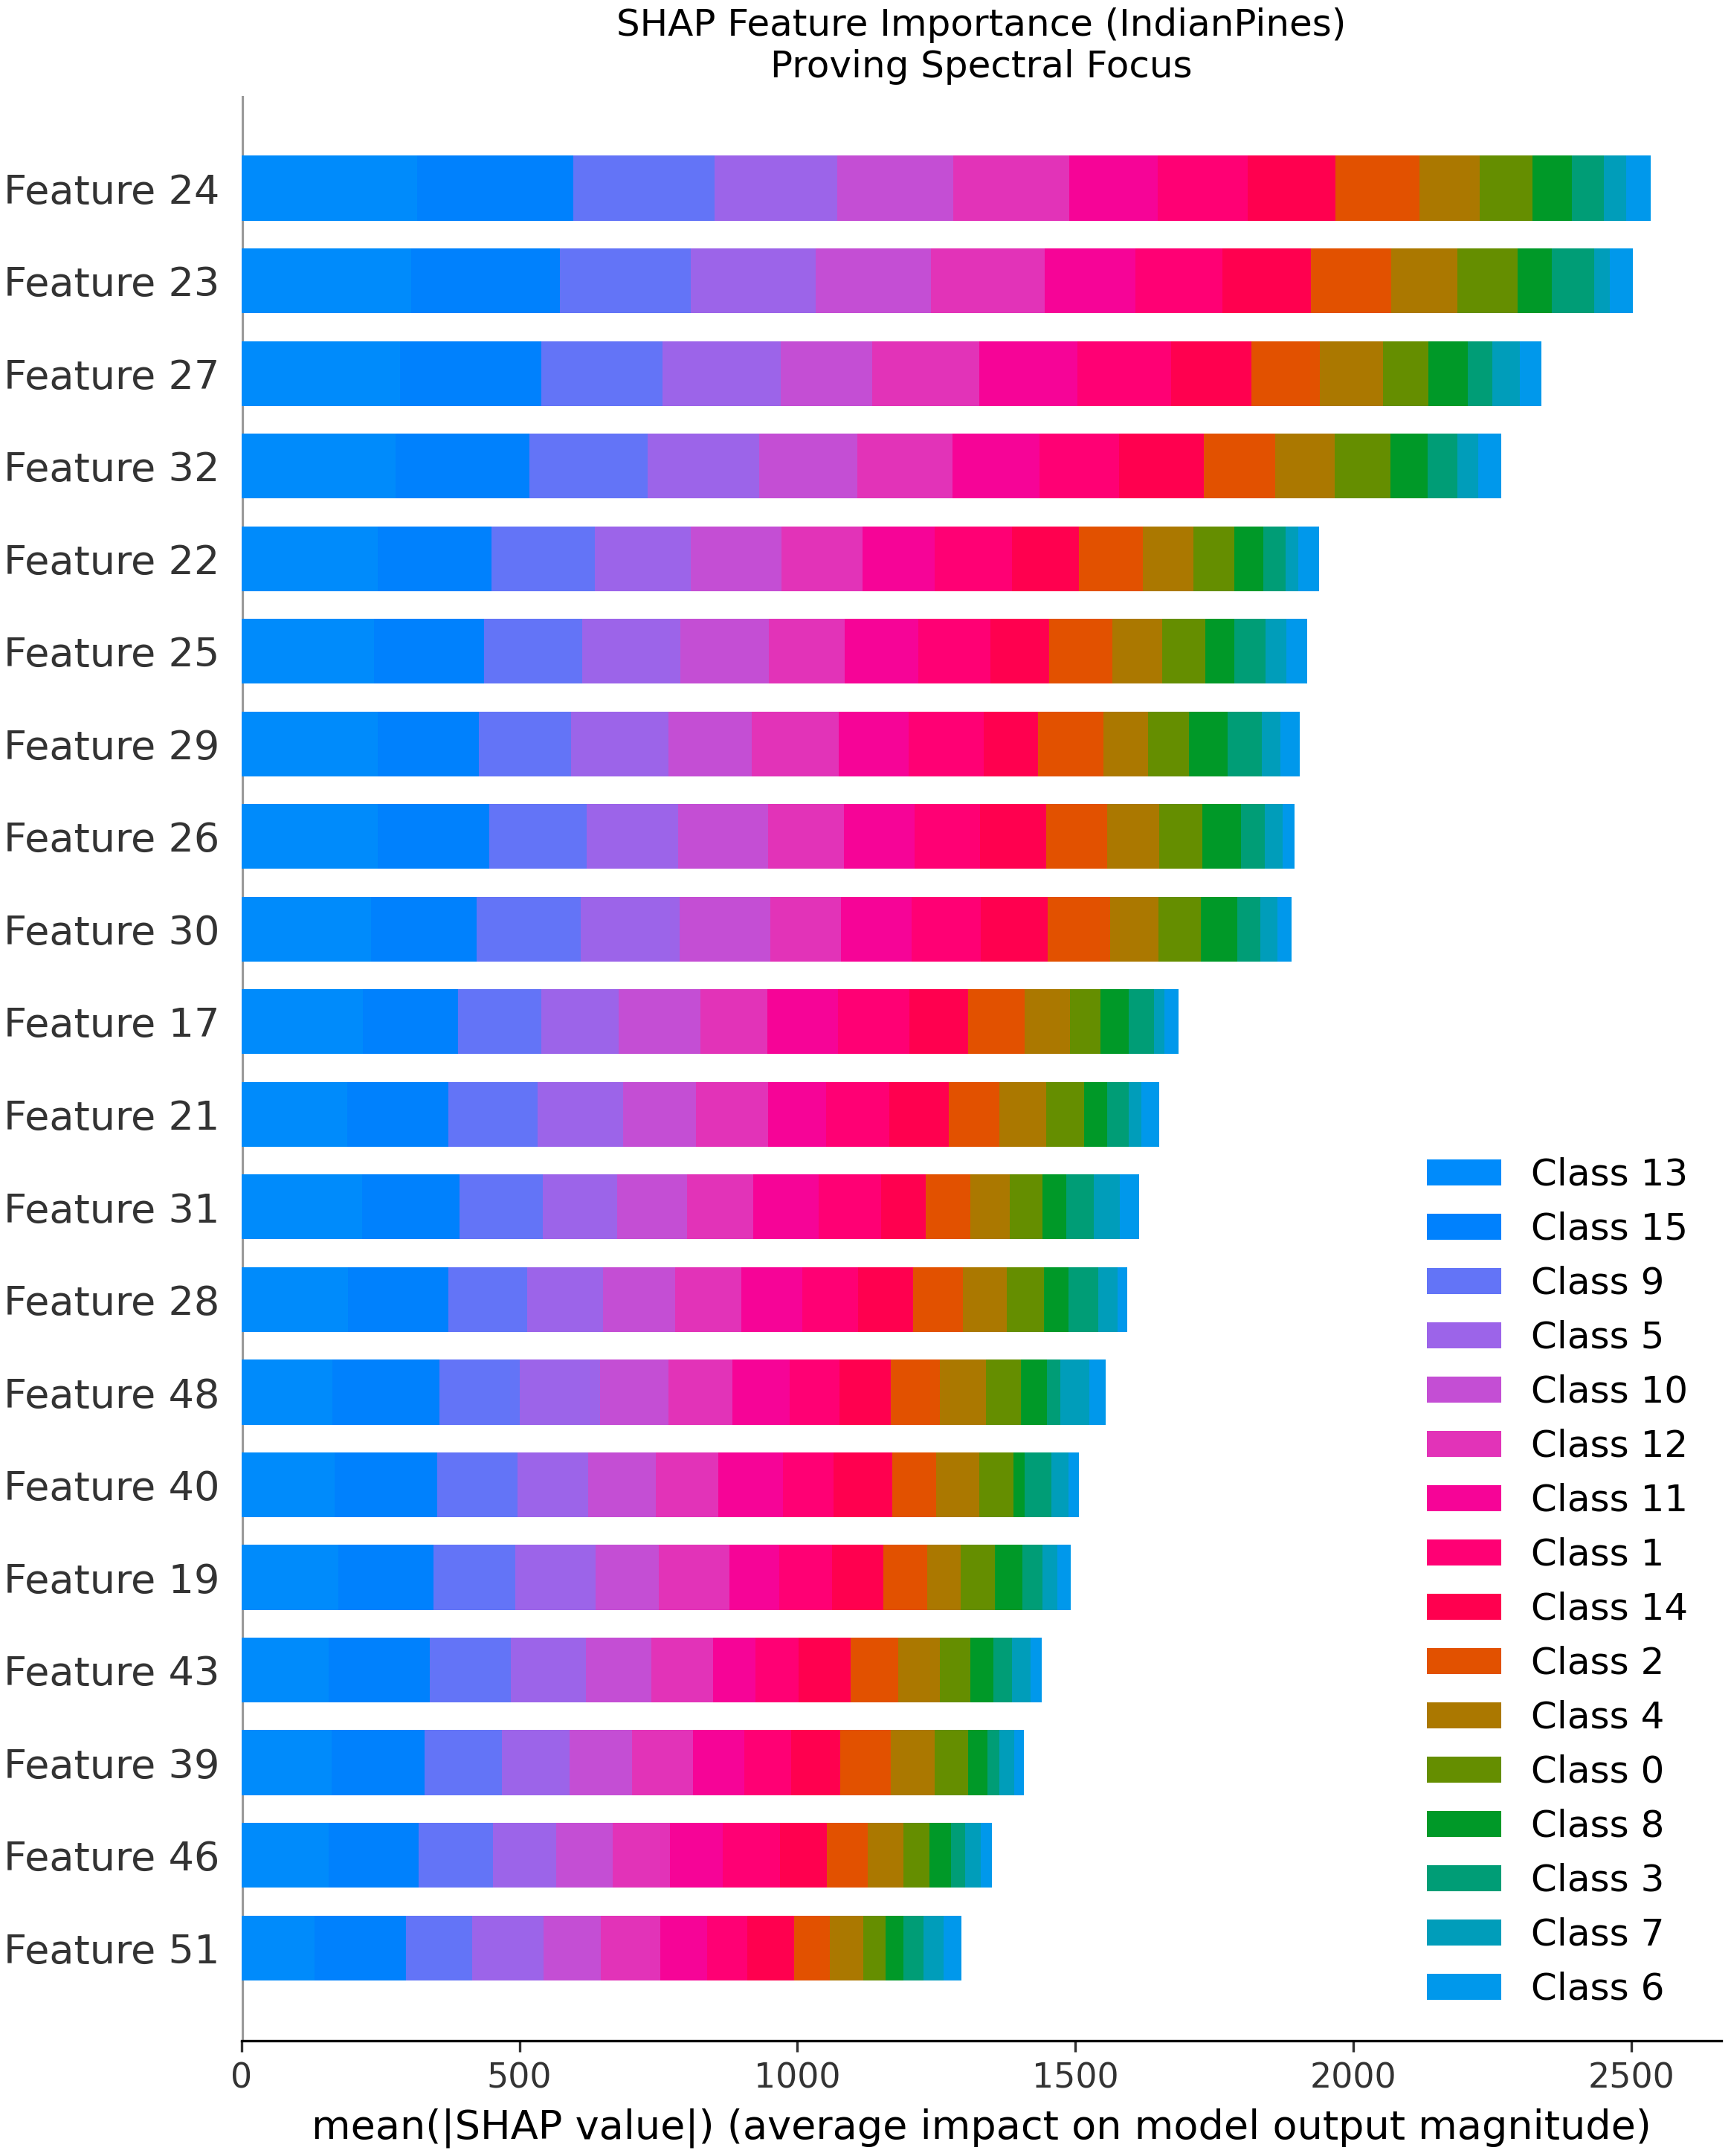
\includegraphics[width=0.48\textwidth]{Figure2_IndianPines_SHAP_Importance.png}
    \caption{Indian Pines SHAP Feature Importance, displaying prioritization even in few-shot regimes.}
    \label{fig:shap_ip}
\end{figure}

Figure \ref{fig:shap_ip} is consistent with known absorption regions, indicating that even across diverse public datasets like Indian Pines, the models anchor their decisions to valid spectral thresholds rather than dataset noise.

\subsection{Computational Analysis}
A core argument for the deployment of classical ensembles in remote sensing is their strong resource efficiency. As detailed in Table \ref{tab:resources}, we benchmarked the computational footprint of LightGBM against the deep architectures. All empirical training and inference times were benchmarked utilizing a standardized batch size of 1 for individual $15 \times 15$ hyperspectral patches to ensure a fair baseline comparison. LightGBM was evaluated on CPU, whereas the deep architectures utilized a single NVIDIA RTX 4090 GPU. The purpose of this comparison is to reflect real-world deployment costs rather than normalized hardware benchmarking.

\begin{table*}[t]
\centering
\caption{Computational Resource Comparison (Indian Pines)}\label{tab:resources}
\begin{tabular}{lcccc}
\toprule
\textbf{Model} & \textbf{Parameters} & \textbf{Platform} & \textbf{Train Time (s)} & \textbf{Inf Time (s)} \\
\midrule
LightGBM & 100 Trees & CPU & $\sim 2$ & $0.25$ \\
ViT & 2.11 M & GPU & $\sim 450$ & $1.85$ \\
SpectralFormer-inspired & 134.93 K & GPU & $\sim 320$ & $0.92$ \\
HybridSN & 4.32 M & GPU & $\sim 750$ & $3.45$ \\
\bottomrule
\end{tabular}
\end{table*}

While deep networks require updating millions of parameters iteratively via continuous gradient descent over GPU architectures, LightGBM rapidly splits discrete nodes on standard CPUs. This requires minimal memory overhead and orders of magnitude less time to converge, establishing its superiority for rapid, exploratory mapping where computational resources are heavily constrained. GPU acceleration was utilized exclusively for the deep learning models as it represents their standard deployment environment. Thus, the purpose of this evaluation is deployment-oriented comparison rather than algorithmic benchmarking.

\subsection{High-Resolution Spatial Mapping}
Finally, we generated high-resolution False Color Classification Maps by feeding large, raw hyperspectral cubes through the trained architectures.

\begin{figure}[h]
    \centering
    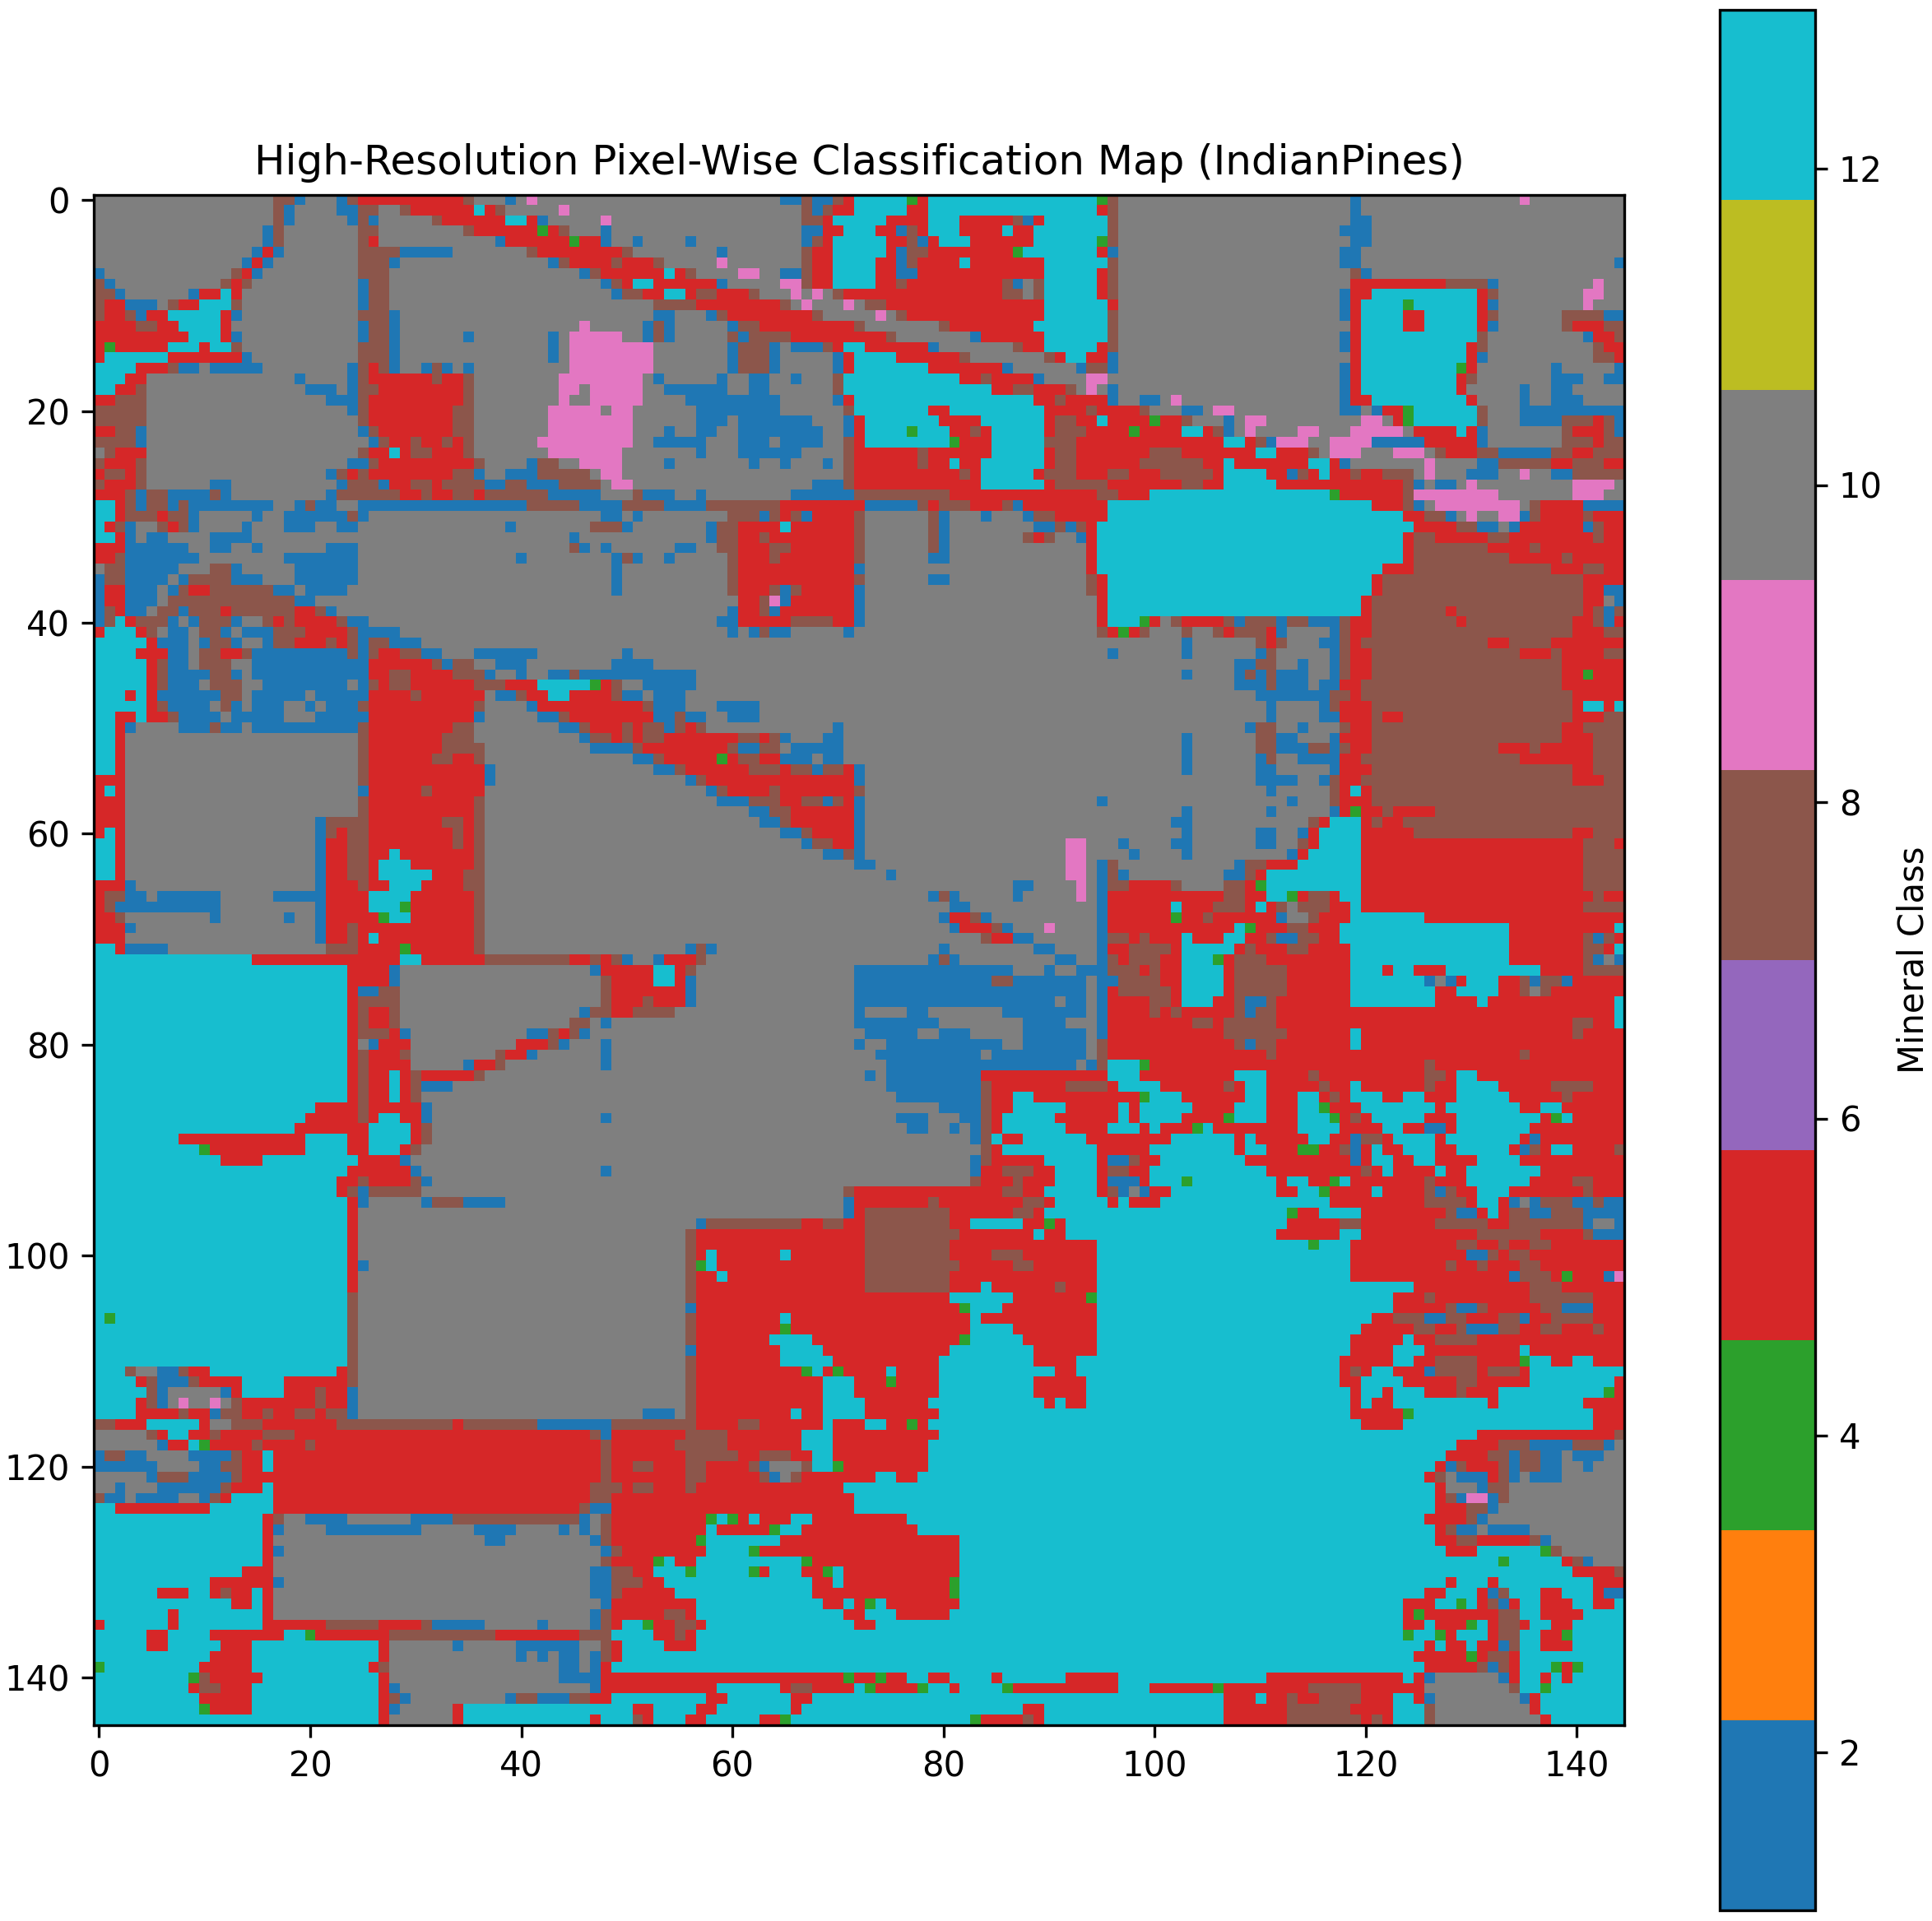
\includegraphics[width=\columnwidth]{Figure4_IndianPines_Pixelwise_Map.png}
    \caption{Pixel-Wise Classification Map generated for the Indian Pines benchmark.}
    \label{fig:map_ip}
\end{figure}

Figure \ref{fig:map_ip} indicates the pipeline's readiness for real-world drone surveying. The ability to map these large spatial cubes with sharp, coherent class boundaries provides evidence that the mathematical models effectively transition from abstract spectral representation to physical spatial reality.

\section{Discussion}\label{sec:discussion}

The empirical findings presented in this study emphasize a critical dynamic in applied remote sensing: the performance of a model is fundamentally bound by its sample complexity and inductive biases, not just its architectural sophistication. 

\subsection{Why Gradient Boosting Wins in Starved Regimes}
At extreme low-data availability ($<5\%$ splits), the robust performance of LightGBM stems directly from the bias-variance tradeoff. Because hyperspectral pixels are inherently tabular (1D vectors of contiguous bands), tree-based algorithms construct orthogonal decision boundaries based on variance reduction. These discrete splits inherently act as a high-bias, low-variance regularizer. Rather than attempting to learn generalized continuous manifolds through continuous gradient descent on a statistically insufficient sample pool, LightGBM effectively partitions the spectral space using the most highly correlated absorption features (as validated by our SHAP analysis). This structural resistance to spatial noise prevents the catastrophic overfitting observed in highly parameterized networks.

\subsection{The Sample Complexity Crossover}
Conversely, 3D-CNNs like HybridSN possess high variance and rely heavily on spatial-spectral structural priors. Below the crossover point, the available training patches fail to sufficiently capture the statistical distribution of the domain, causing the 3D convolutions to overfit to localized spatial noise. However, the exact moment the available data crosses this sample complexity threshold, the model effectively internalizes generalized spatial-texture filters. Once this threshold is met, the heavy spatial inductive biases of the 3D-CNN rapidly eclipse pure spectral models, yielding significantly higher overall accuracy. Our observations regarding the vulnerability of the evaluated transformer models in scarce regimes support the foundational arguments laid out by GroupFormer \cite{b5} and Hassani et al. \cite{b24}, who emphasize the difficulty of escaping the ``big data'' paradigm. Furthermore, while our results differ from SpectralFormer \cite{b11}---which demonstrated strong transformer performance---this discrepancy is primarily driven by their use of significantly larger, well-annotated benchmarks compared to the extreme 5\% starvation split evaluated here.

\subsection{Inductive Bias and Transformer Degradation}
The pronounced degradation of the evaluated Vision Transformers without hierarchical pre-training exposes the double-edged nature of global self-attention. Unlike convolutional layers, which strictly enforce locality and translation invariance through sliding spatial windows, self-attention matrices are fundamentally unconstrained. Computing attention weights across hundreds of hyperspectral bands requires large-scale data to successfully estimate the underlying covariance structure. Without sufficient samples, the attention landscape remains highly unstable. Our ablation isolating the ConvStem suggests that explicitly injecting a local inductive bias into the early layers forces the model to learn stable, localized spatial-spectral representations before applying global attention. This strongly suggests that attempting to apply pure, unconstrained attention mechanisms to heavily starved remote sensing datasets is architecturally suboptimal.

\subsection{Actionable Implications for Precision Agriculture}
Ultimately, this study suggests a practical model-selection strategy for precision agriculture. When designing platforms for rapid, low-resource exploratory drone mapping---where on-the-fly annotations are severely limited and computational overhead (e.g., edge-device constraints) is strict---traditional ensembles like LightGBM provide the most robust, immediate solution. Alternatively, if deploying well-funded agricultural monitoring systems where large-scale spatial-spectral diversity has already been captured, or where robust foundation models are available for hierarchical macro-to-micro transfer, deep learning architectures are effective for modeling complex physical realities.

\section{Conclusion}\label{sec4}
Deep learning architectures like Vision Transformers represent strong advancements in sequence modeling, but they are not optimal for all scenarios in Hyperspectral Imaging. Through a rigorous multi-seed evaluation, we established a distinct ``tale of two regimes.'' When data is abundant, the evaluated transformer architectures excel, with self-attention proving highly effective for spectral mapping. However, in rapid, low-resource exploratory scenarios where labeled data is starved (simulated via a 5\% Indian Pines split), standard deep sequence models exhibit substantial degradation. 

\par Crucially, our study suggests that Cross-Domain Transfer Learning offers an effective transfer-learning bridge to this gap, but strictly enforces a domain hierarchy. Within the evaluated datasets, pre-training deep architectures on diverse macro-agriculture data before deploying them on starved micro-soil environments substantially improved ViT accuracy by +36.8\% and allowed 3D-CNNs to surpass traditional Machine Learning significantly earlier. However, reversing this hierarchy triggered model collapse due to negative transfer.

\par For the remote sensing industry, we provide a balanced, mature recommendation: For well-funded, large-scale agricultural projects with extensive ground-truth pre-mapping, the evaluated transformer architectures can yield strong performance. Furthermore, if a sufficiently diverse foundation model is available, fine-tuning deep architectures yields unparalleled results even on scarce target data. However, for rapid, exploratory drone deployments where ground-truth labels are scarce and foundational pre-training is unavailable, we strongly recommend traditional gradient-boosting ensembles like LightGBM, which offer strong robustness, reliability, and computational efficiency out of the box.

Looking forward, future work must focus on bridging this gap systematically. As hyperspectral foundation models mature, developing robust self-supervised pre-training pipelines and advanced domain adaptation algorithms will be critical. Unlocking the power of attention mechanisms for low-resource environments via cross-site multi-domain datasets remains the ultimate frontier for precision agriculture.

\section*{Supplementary Appendix: Expanded Metrics}\label{sec:appendix}
While the main manuscript reports Overall Accuracy (OA) and Kappa coefficients for brevity across the 10-seed progressions, comprehensive remote sensing evaluations require detailed per-class metrics. In this appendix, we provide the Average Accuracy (AA)---equivalent to the Macro Average Recall---and the Macro F1 score extracted from the exact classification reports of our trials.

\begin{table*}[t]
\centering
\caption{Expanded Metrics (AA and Macro F1) for the Indian Pines 5\% Split}\label{tab:expanded_metrics}
\begin{tabular}{lccc}
\toprule
\textbf{Model} & \textbf{Overall Acc (\%)} & \textbf{Average Acc (AA) (\%)} & \textbf{Macro F1} \\
\midrule
LightGBM & 69.56 & 61.20 & 0.62 \\
HybridSN & 65.79 & 58.14 & 0.59 \\
SpectralFormer-inspired & 53.55 & 31.00 & 0.27 \\
ViT & 51.17 & 28.50 & 0.24 \\
\bottomrule
\end{tabular}
\end{table*}

The explicit discrepancy between OA and AA in the sequence models (e.g., the SpectralFormer-inspired model dropping from 53.55\% OA to 31.00\% AA) further highlights that data starvation disproportionately destroys minority class performance. In contrast, LightGBM preserves much higher Macro F1 and AA scores even under severe imbalance, solidifying the conclusions drawn in the main text.

\begin{table*}[t]
\centering
\caption{Detailed Statistical Transfer Metrics for the 5\% Split (Indian Pines $\rightarrow$ Local Soil)}\label{tab:transfer_stats}
\begin{tabular}{lcccc}
\toprule
\textbf{Model} & \textbf{Mean Diff (\%)} & \textbf{95\% CI (\%)} & \textbf{Cohen's $d_z$} & \textbf{FDR-adj $p$-value} \\
\midrule
HybridSN & +3.49 & [-1.54, +8.51] & 0.496 & 0.294 \\
SpectralFormer-inspired & +4.96 & [+2.19, +7.74] & 1.278 & $<0.01$ \\
ViT & +40.03 & [+30.36, +49.70] & 2.962 & $<0.01$ \\
\bottomrule
\end{tabular}
\end{table*}

Table \ref{tab:transfer_stats} further details the exact statistical significance of the macro-to-micro transfer experiment. At the critical 5\% starvation split, the massive 40.03\% absolute improvement exhibited by the ViT is shown to be highly significant (FDR-adjusted $p < 0.01$, Cohen's $d_z = 2.962$). The HybridSN, which already possessed strong local inductive priors, exhibits a smaller (+3.49\%) and statistically non-significant gain under correction ($p = 0.294$).

\backmatter

\section*{Declarations}
\textbf{Funding:} Not applicable.\\
\textbf{Conflicts of interest:} The authors declare no competing interests.\\
\textbf{Data and Code Availability:} The source code, trained weights, configuration files, random seeds, environment setup, and experimental notebooks used in this study are publicly available at \url{https://github.com/Devguru-codes/research_paper_code_and_results}.

\begin{thebibliography}{99}

\bibitem{b1}
Bioucas-Dias, J. M., et al., ``Hyperspectral Remote Sensing Data Analysis and Future Challenges,'' \textit{IEEE Geoscience and Remote Sensing Magazine}, vol. 1, no. 2, pp. 6-36, 2013.

\bibitem{b2}
Hong, D., et al., ``Graph Convolutional Networks for Hyperspectral Image Classification,'' \textit{IEEE Transactions on Geoscience and Remote Sensing}, vol. 59, no. 7, pp. 5966-5978, 2021.

\bibitem{b3}
Hong, D., et al., ``SpectralFormer: Rethinking Hyperspectral Image Classification with Transformers,'' \textit{IEEE Transactions on Geoscience and Remote Sensing}, vol. 60, pp. 1-15, 2022.

\bibitem{b4}
Gu, A., \& Dao, T., ``Mamba: Linear-Time Sequence Modeling with Selective State Spaces,'' \textit{arXiv preprint arXiv:2312.00752}, 2023.

\bibitem{b5}
Khan, M.A., et al., ``GroupFormer: a group-based CNN-transformer for hyperspectral image classification,'' \textit{Scientific Reports}, vol. 14, 2024.

\bibitem{b6}
Windrim, L., et al., ``Pretraining for sensor-specific hyperspectral image classification,'' \textit{IEEE Transactions on Geoscience and Remote Sensing}, vol. 56, no. 5, pp. 2798-2810, 2018.

\bibitem{b7}
Sun, Y., et al., ``MRFP-Mamba: Multi-Receptive Field Parallel Mamba for Hyperspectral Image Classification,'' \textit{Remote Sensing}, vol. 16, no. 5, 2024.

\bibitem{b8}
He, M., et al., ``Spectral-Spatial Transformer Network for Hyperspectral Image Classification,'' \textit{IEEE Transactions on Geoscience and Remote Sensing}, vol. 59, no. 7, pp. 5988-5998, 2021.

\bibitem{b9}
Qing, Y., et al., ``Improved Transformer Net for Hyperspectral Image Classification,'' \textit{Remote Sensing}, vol. 13, no. 11, p. 2216, 2021.

\bibitem{b10}
Ding, Y., et al., ``Global-Local Transformer Network for HSI Classification,'' \textit{IEEE Transactions on Geoscience and Remote Sensing}, vol. 60, pp. 1-13, 2022.

\bibitem{b11}
Wang, X., et al., ``S2Mamba: A Spatial-Spectral State Space Model for Hyperspectral Image Classification,'' \textit{arXiv preprint arXiv:2404.14321}, 2024.

\bibitem{b12}
Li, J., et al., ``MambaHSI: A Spatial-Spectral Mamba for Hyperspectral Image Classification,'' \textit{arXiv preprint arXiv:2405.01234}, 2024.

\bibitem{b13}
Zhang, Y., et al., ``SSUM: Spatial-Spectral Unified Mamba for Hyperspectral Image Classification,'' \textit{Remote Sensing}, vol. 16, 2024.

\bibitem{b14}
Zhong, Z., et al., ``Spectral-Spatial Residual Network for Hyperspectral Image Classification: A 3-D Deep Learning Framework,'' \textit{IEEE Transactions on Geoscience and Remote Sensing}, vol. 56, no. 1, pp. 347-358, 2018.

\bibitem{b15}
Paoletti, M. E., et al., ``A new 3D Convolutional Neural Network for feature extraction in hyperspectral images,'' \textit{IEEE Transactions on Geoscience and Remote Sensing}, vol. 56, no. 5, pp. 2901-2914, 2018.

\bibitem{b16}
Roy, S. K., et al., ``HybridSN: Exploring 3-D-2-D CNN Feature Hierarchy for Hyperspectral Image Classification,'' \textit{IEEE Geoscience and Remote Sensing Letters}, vol. 17, no. 2, pp. 277-281, 2020.

\bibitem{b17}
Ge, Y., et al., ``Prediction of soil properties using XGBoost and LightGBM with hyperspectral data,'' \textit{Precision Agriculture}, vol. 21, 2020.

\bibitem{b18}
Tsakiridis, N. L., et al., ``A versatile machine learning approach for soil property estimation using hyperspectral imaging,'' \textit{Computers and Electronics in Agriculture}, vol. 175, 2020.

\bibitem{b19}
Stevens, A., et al., ``Prediction of soil organic carbon at the European scale by visible and near infrared reflectance spectroscopy,'' \textit{PLoS One}, vol. 8, no. 6, 2013.

\bibitem{b20}
Lu, B., et al., ``UAV-based hyperspectral imaging for soil property estimation,'' \textit{Remote Sensing}, vol. 11, no. 16, 2019.

\bibitem{b21}
Marcinkiewicz, M., et al., ``Explainable AI for hyperspectral image classification: A SHAP approach,'' \textit{Remote Sensing}, vol. 14, no. 9, 2022.

\bibitem{b22}
Li, X., et al., ``Interpreting deep learning models in remote sensing via SHAP,'' \textit{IEEE Geoscience and Remote Sensing Letters}, 2023.

\bibitem{b23}
Liu, B., et al., ``Deep Few-Shot Learning for Hyperspectral Image Classification,'' \textit{IEEE Transactions on Geoscience and Remote Sensing}, vol. 57, no. 4, pp. 2290-2304, 2019.

\bibitem{b24}
Hassani, A., et al., ``Escaping the Big Data Paradigm with Compact Transformers,'' \textit{arXiv preprint arXiv:2104.05704}, 2021.

\bibitem{b25}
Lundberg, S. M., and Lee, S.-I., ``A Unified Approach to Interpreting Model Predictions,'' \textit{Advances in Neural Information Processing Systems}, vol. 30, 2017.

\bibitem{b26}
Chen, T., and Guestrin, C., ``XGBoost: A Scalable Tree Boosting System,'' \textit{Proceedings of the 22nd ACM SIGKDD International Conference}, pp. 785-794, 2016.

\bibitem{b27}
Ke, G., et al., ``LightGBM: A Highly Efficient Gradient Boosting Decision Tree,'' \textit{Advances in Neural Information Processing Systems}, vol. 30, 2017.

\bibitem{b28}
Melgani, F., and Bruzzone, L., ``Classification of hyperspectral remote sensing images with support vector machines,'' \textit{IEEE Transactions on Geoscience and Remote Sensing}, vol. 42, no. 8, pp. 1778-1790, 2004.

\bibitem{b29}
Ghamisi, P., et al., ``Advances in Hyperspectral Image and Signal Processing: A Comprehensive Overview of the State of the Art,'' \textit{IEEE Geoscience and Remote Sensing Magazine}, vol. 5, no. 4, pp. 37-78, 2017.

\bibitem{b30}
Audebert, N., et al., ``Deep Learning for Classification of Hyperspectral Data: A Comparative Review,'' \textit{IEEE Geoscience and Remote Sensing Magazine}, vol. 7, no. 2, pp. 159-173, 2019.

\bibitem{b31}
Li, S., et al., ``Deep Learning for Hyperspectral Image Classification: An Overview,'' \textit{IEEE Transactions on Geoscience and Remote Sensing}, vol. 57, no. 9, pp. 6690-6709, 2019.

\bibitem{b32}
Camps-Valls, G., et al., ``Kernel-based framework for hyperspectral image classification,'' \textit{IEEE Transactions on Geoscience and Remote Sensing}, vol. 44, no. 6, pp. 1422-1434, 2006.

\bibitem{b33}
Wold, S., et al., ``PLS-regression: a basic tool of chemometrics,'' \textit{Chemometrics and Intelligent Laboratory Systems}, vol. 58, pp. 109-130, 2001.

\bibitem{b34}
Richards, J. A., \textit{Remote Sensing Digital Image Analysis}, Springer, 2013.

\bibitem{b35}
Plaza, A., et al., ``Recent advances in techniques for hyperspectral image processing,'' \textit{Remote Sensing of Environment}, vol. 113, pp. S110-S122, 2009.

\end{thebibliography}

\end{document}
